\documentclass[aspectratio=1610]{beamer}
\usetheme{alxprc}

\usepackage{packages}
\usepackage{pgfplots}
\usepackage[italic]{hepnames}

\title{WG5 Summary}
\subtitle{Physics with Heavy Flavours}
\date{%
  Friday $ 7^{\text{th}}$ April 2017\\
  \href{https://indico.cern.ch/event/568360/}{DIS 2017, Birmingham, UK}
}

\author[WG 5]{%
  \texorpdfstring{%
    Rhorry Gauld${}^{1}$,
    Andrea Giammanco${}^{2}$,
    \structure{Alex Pearce}${}^{3}$\\
    {\footnotesize ${}^{1}$ETH Z\"{u}rich, ${}^{2}$UCLouvain, ${}^{3}$CERN}
  }{%
    Rhorry Gauld (ETH Zurich),
    Andrea Giammanco (UCLouvain),
    Alex Pearce (CERN)
  }
}

\newcommand{\righttitle}[1]{\hspace{0pt plus 1 filll}{\footnotesize #1}}

\begin{document}

\begin{frame}
  \begin{center}
    \usebeamerfont{title}{\usebeamercolor[fg]{title}\inserttitle}\par
    \usebeamerfont{subtitle}{\insertsubtitle}\par
    \bigskip
    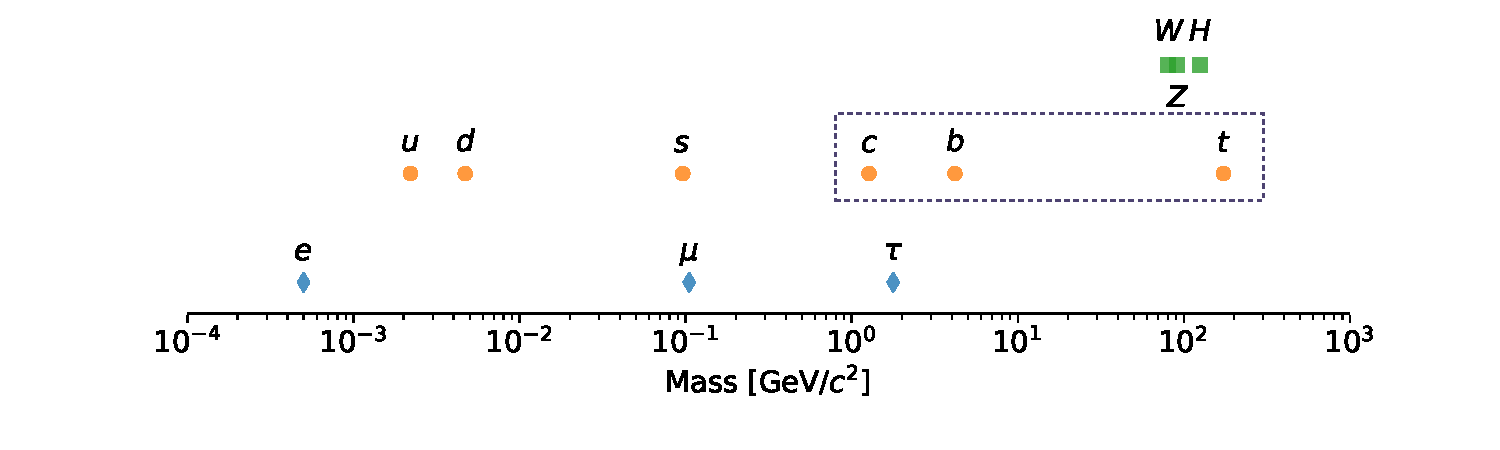
\includegraphics[width=\textwidth]{masses_wide}\par
    \bigskip
    \usebeamerfont{author}\insertauthor\par
    \bigskip
    \usebeamerfont{date}\insertdate\par
  \end{center}
\end{frame}

\begin{frame}{What did we talk about?}
  \begin{enumerate}
    \item Top quark pairs
    \item Single top production and properties
    \item Top quark mass
    \item Beauty and charm quark production
    \item Heavy flavour measurements for PDF fits (joint with WG1)
    \item Properties of \B and \D hadrons
    \item Exotic states
    \item Quarkonia
  \end{enumerate}
\end{frame}

\section{Heavy flavour cross-sections in \pp\ collisions}
\begin{frame}{Heavy flavour cross-sections in \pp\ collisions}
  \begin{columns}
    \begin{column}{0.5\textwidth}
      \begin{center}
        \feynmandiagram [large, horizontal=a to b] {%
  i1 [particle=\(\Pgluon\)] -- [gluon] a -- [gluon] i2 [particle=\(\Pgluon\)],
  a -- [gluon] b,
  f1 [particle=\(\APquark\)] -- [fermion] b -- [fermion] f2 [particle=\(\Pquark\)],
};

      \end{center}
    \end{column}

    \begin{column}{0.5\textwidth}
      \begin{center}
        \feynmandiagram [large, layered layout, horizontal=a to b] {
  % Draw the top and bottom lines
  i1 [particle=\(\Pgluon\)] -- [gluon] a -- [anti fermion] b [particle=\(\APquark\)],
  i2 [particle=\(\Pgluon\)] -- [gluon] c -- [fermion] d [particle=\(\Pquark\)],
  % Draw the two internal fermion lines
  { [same layer] a -- [fermion] c },
};

      \end{center}
    \end{column}
  \end{columns}
  \bigskip
  \begin{itemize}
    \item Assume short- and long-distance processes factorise
    \item Test predictions of perturbative QCD
    \item Constrain non-perturbative QCD
    \item Useful for event modelling, MC generator tuning
  \end{itemize}
\end{frame}

\subsection{Top pair production}
\begin{frame}{Top pair production %
              \only<1>{\righttitle{\href{https://indico.cern.ch/event/568360/contributions/2435580/}{Y.\ Yamazaki, M.\ Haleem}}}%
              \only<2>{\righttitle{\href{https://indico.cern.ch/event/568360/contributions/2464600/}{J.\ Gonzalez}}}}
  Top quark is a particularly unique object, \structure{$\mathcal{O}(10^{7})$ \ttbar\ produced} at the LHC so far
  % Heaviest quark
  % Only quark to decay before hadronising
  % Used to constrain parameters like $\alpha_{s}$, $m_{\Ptop}$
  % Can constrain PDFs at high x

  \begin{center}
    \only<1>{%
      \begin{minipage}{0.6\textwidth}
        \begin{tikzpicture}
  \node[anchor=south west, inner sep=0] (image) at (0, 0) {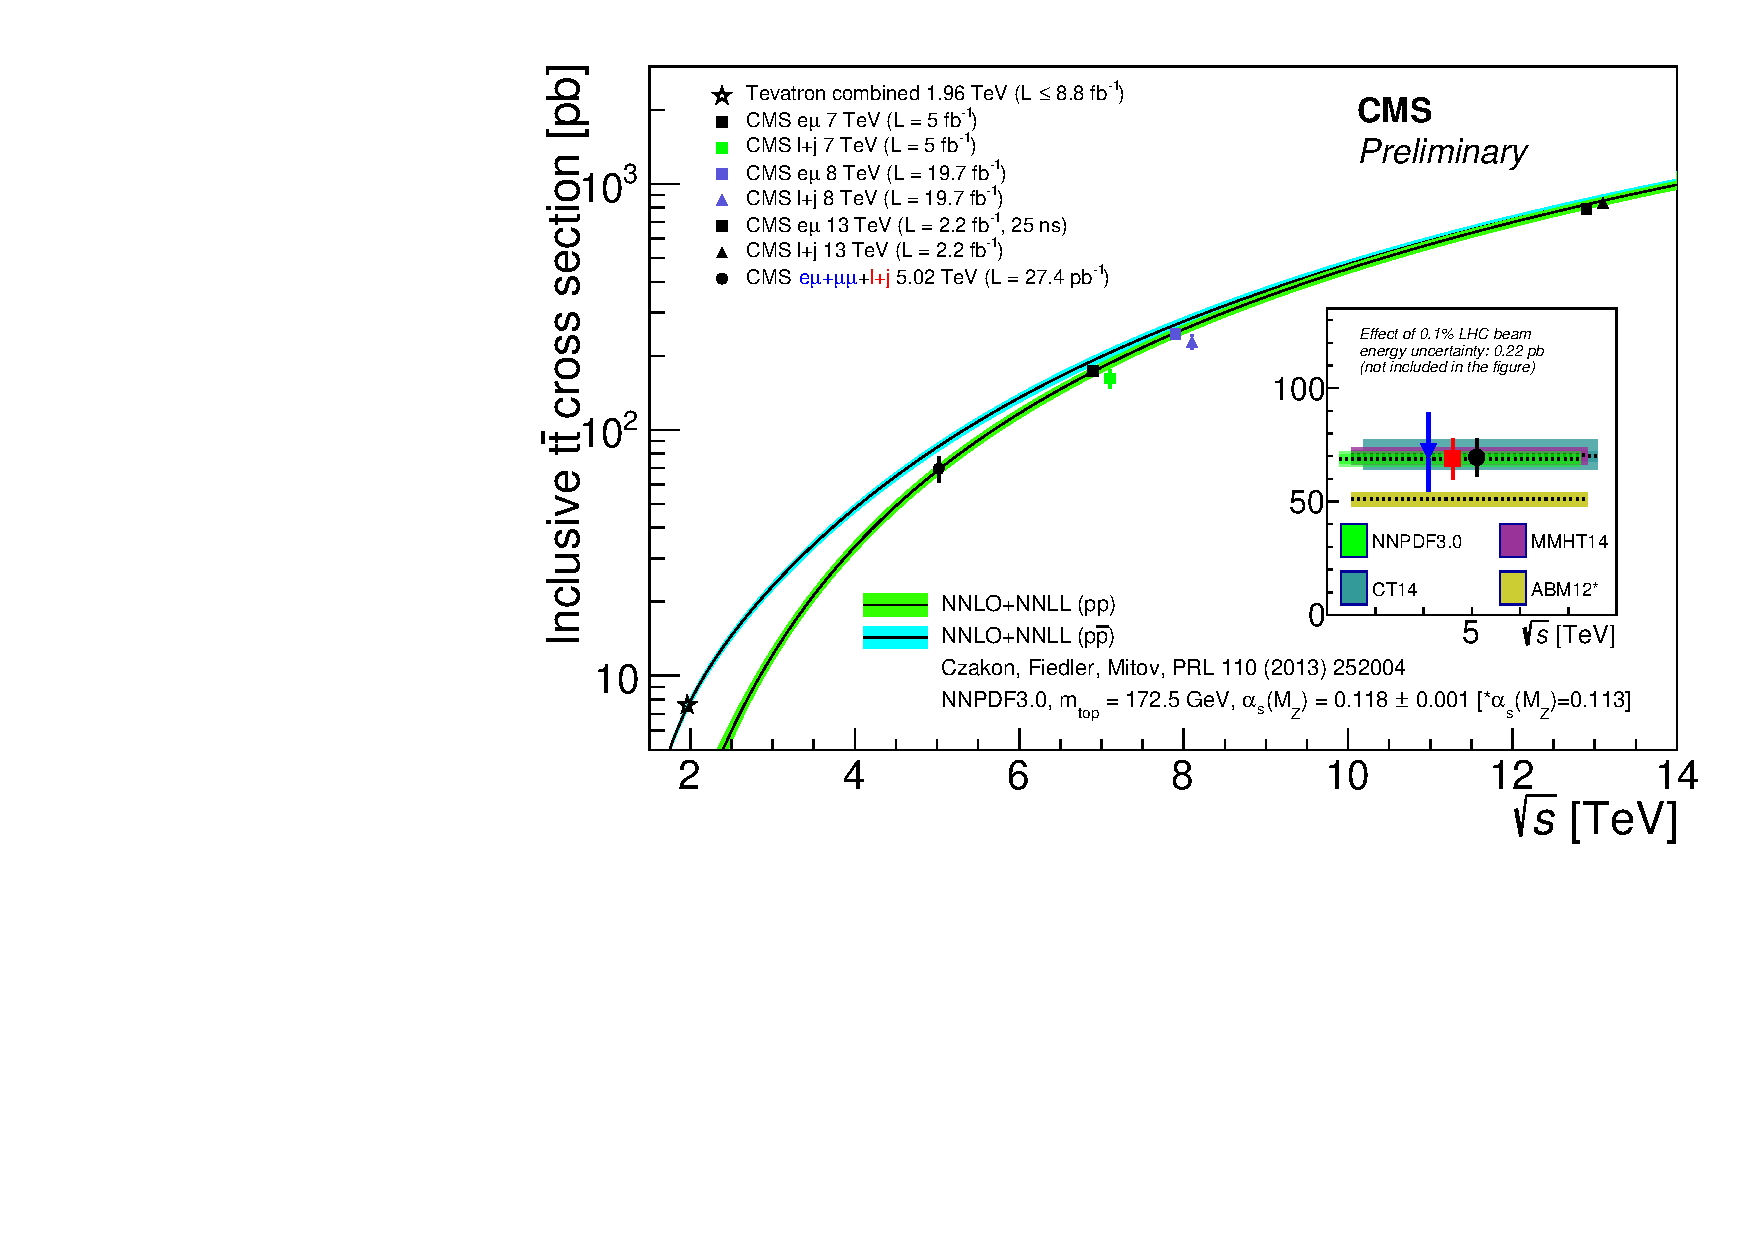
\includegraphics[width=\textwidth]{cms_ttbar_xsec_sqrts_spectrum}};
  \begin{scope}[x={(image.south east)}, y={(image.north west)}]
    % Grid to help find coordinates on the image
    % \draw[step=0.02, gray, very thin] (0, 0) grid (1, 1);
    % Box to cover axis labels
    \draw[thick, color=red!70] (0.345, 0.47) circle (0.4cm);
    % \path[fill=white] (0.02, 0.16) rectangle (0.18, 0.22) node [pos=0.5] {\footnotesize$\theta_{1}$};
  \end{scope}
\end{tikzpicture}

      \end{minipage}

      \structure{New!} Combination of $\sigma(\ttbar)$ at $\sqrts = \SI{5}{\TeV}$
    }
    \only<2>{%
      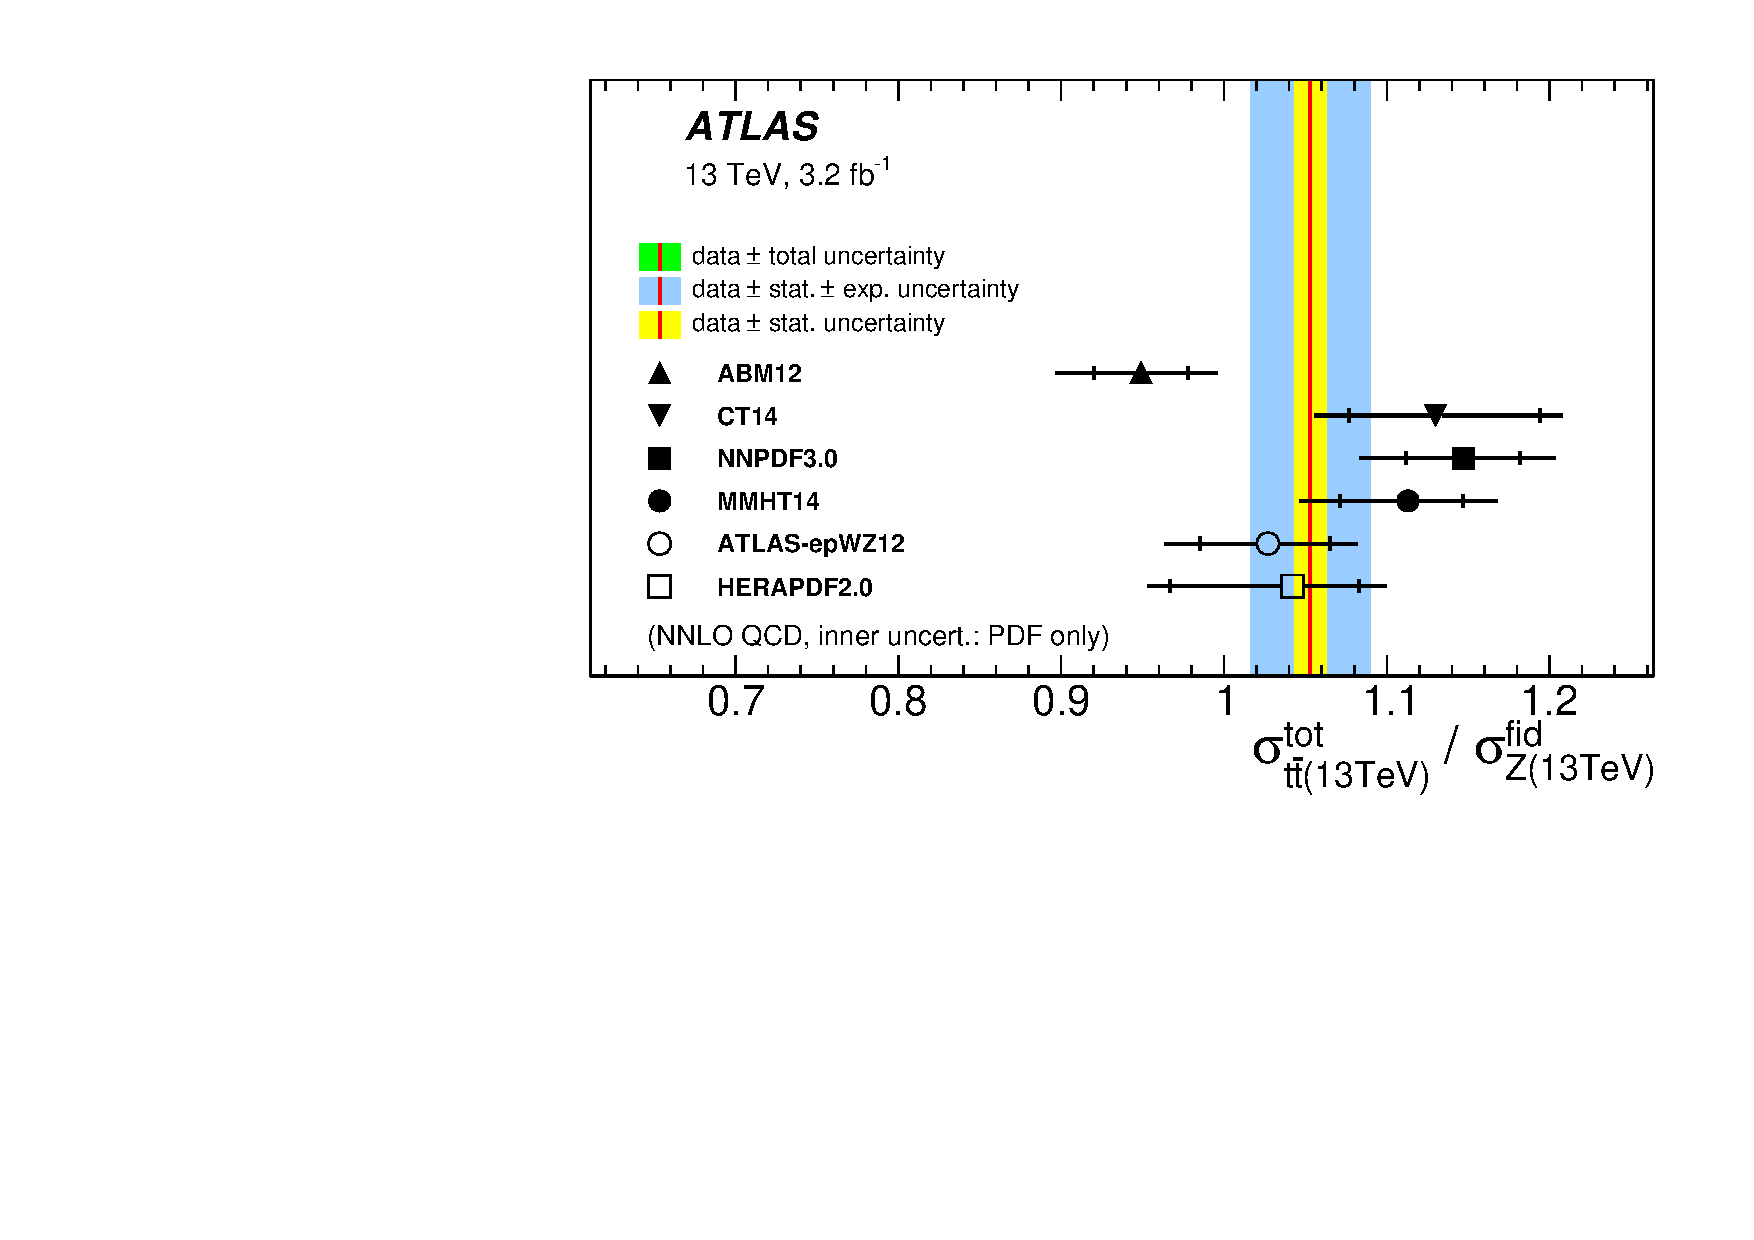
\includegraphics[width=0.6\textwidth]{atlas_ttbar_vs_z_xsec}

      Measurement of $\sigma(\ttbar)/\sigma(\PZ)$ at $\sqrts = \SI{13}{\TeV}$,\\
      sensitive to quark-to-gluon PDF ratio
    }
  \end{center}
\end{frame}

\subsection{Single top production}
\begin{frame}{Single top production%
              \righttitle{\href{https://indico.cern.ch/event/568360/contributions/2435599/<Paste>}{I. Cioar\u{a}}}}
  Single top productions probes electroweak physics\par
  \bigskip
  \structure{Example}: Measure angular asymmetries in $Wtb$ vertex at the parton

  \only<1>{%
    \begin{columns}
      \begin{column}{0.5\textwidth}
        \centering
        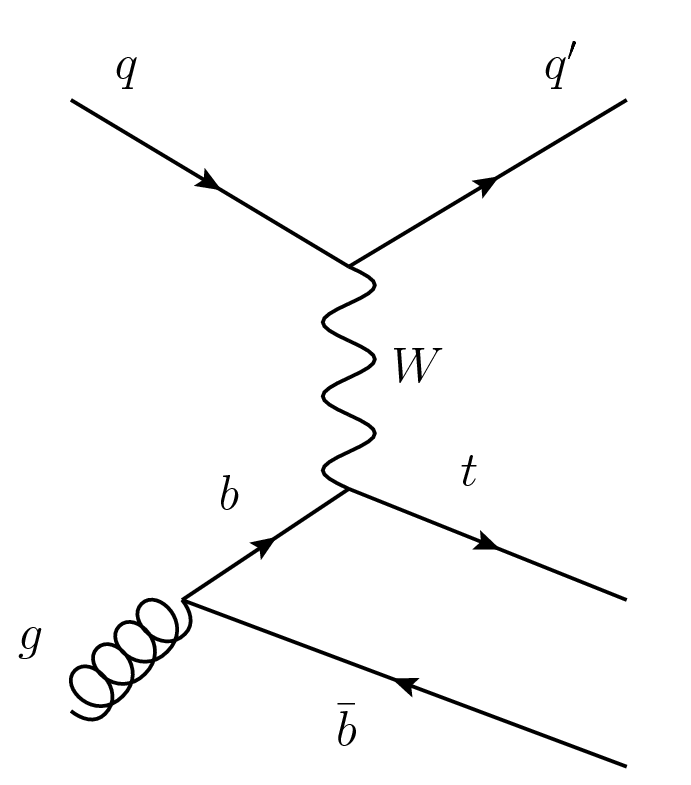
\includegraphics[width=0.55\textwidth]{figures/single_top_t-channel.png}
      \end{column}
      \begin{column}{0.5\textwidth}
        \centering
        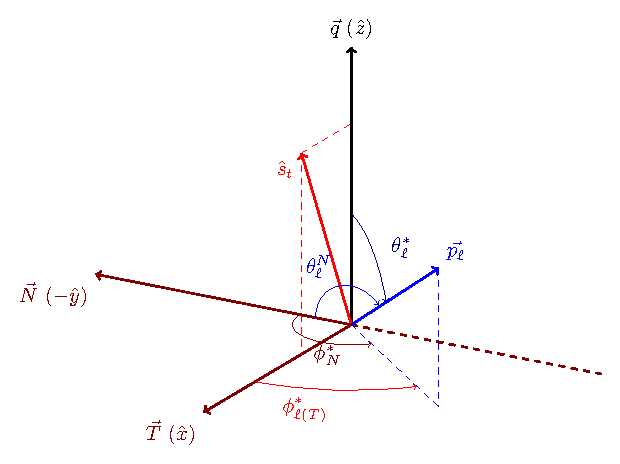
\includegraphics[width=0.9\textwidth]{wtb_angles}
      \end{column}
    \end{columns}

    \bigskip
    \[
      A_{\text{FB}} = \frac{%
        N(\cos{\theta} > 0) - N(\cos{\theta} < 0)
      }{%
        N(\cos{\theta} > 0) + N(\cos{\theta} < 0)
      }
    \]
  }
  \only<2>{%
    \begin{center}
      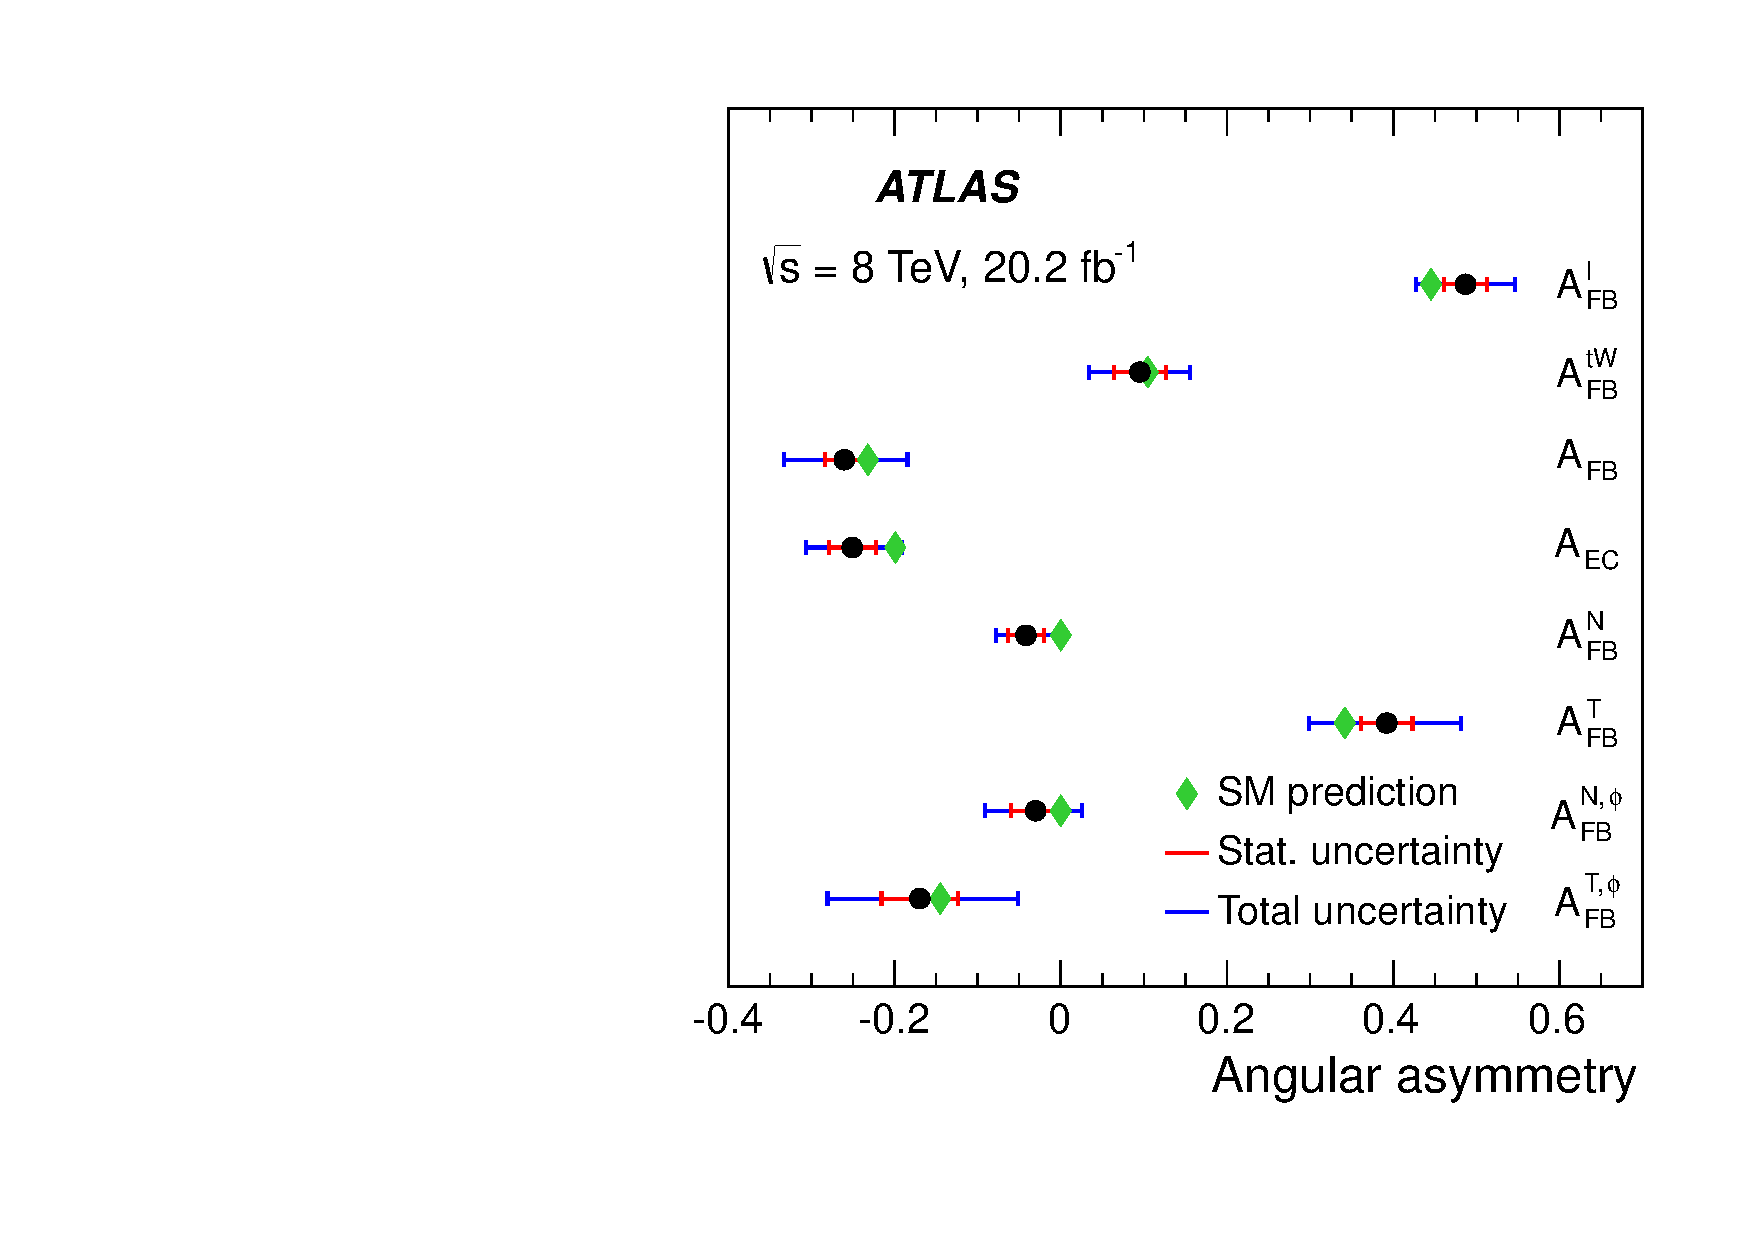
\includegraphics[width=0.5\textwidth]{wtb_results}
    \end{center}
  }
\end{frame}

\subsection{Beauty production}
\begin{frame}{Beauty production%
              \righttitle{%
                \href{https://indico.cern.ch/event/568360/contributions/2471944/}{P.\ Ronchese},
                \href{https://indico.cern.ch/event/568360/contributions/2486101/}{M.\ Boer, X.\ Li}
              }}
  Charm and beauty production can test specific hadronisation schemes

  \bigskip
  \begin{columns}
    \begin{column}{0.4\textwidth}
      \begin{center}
        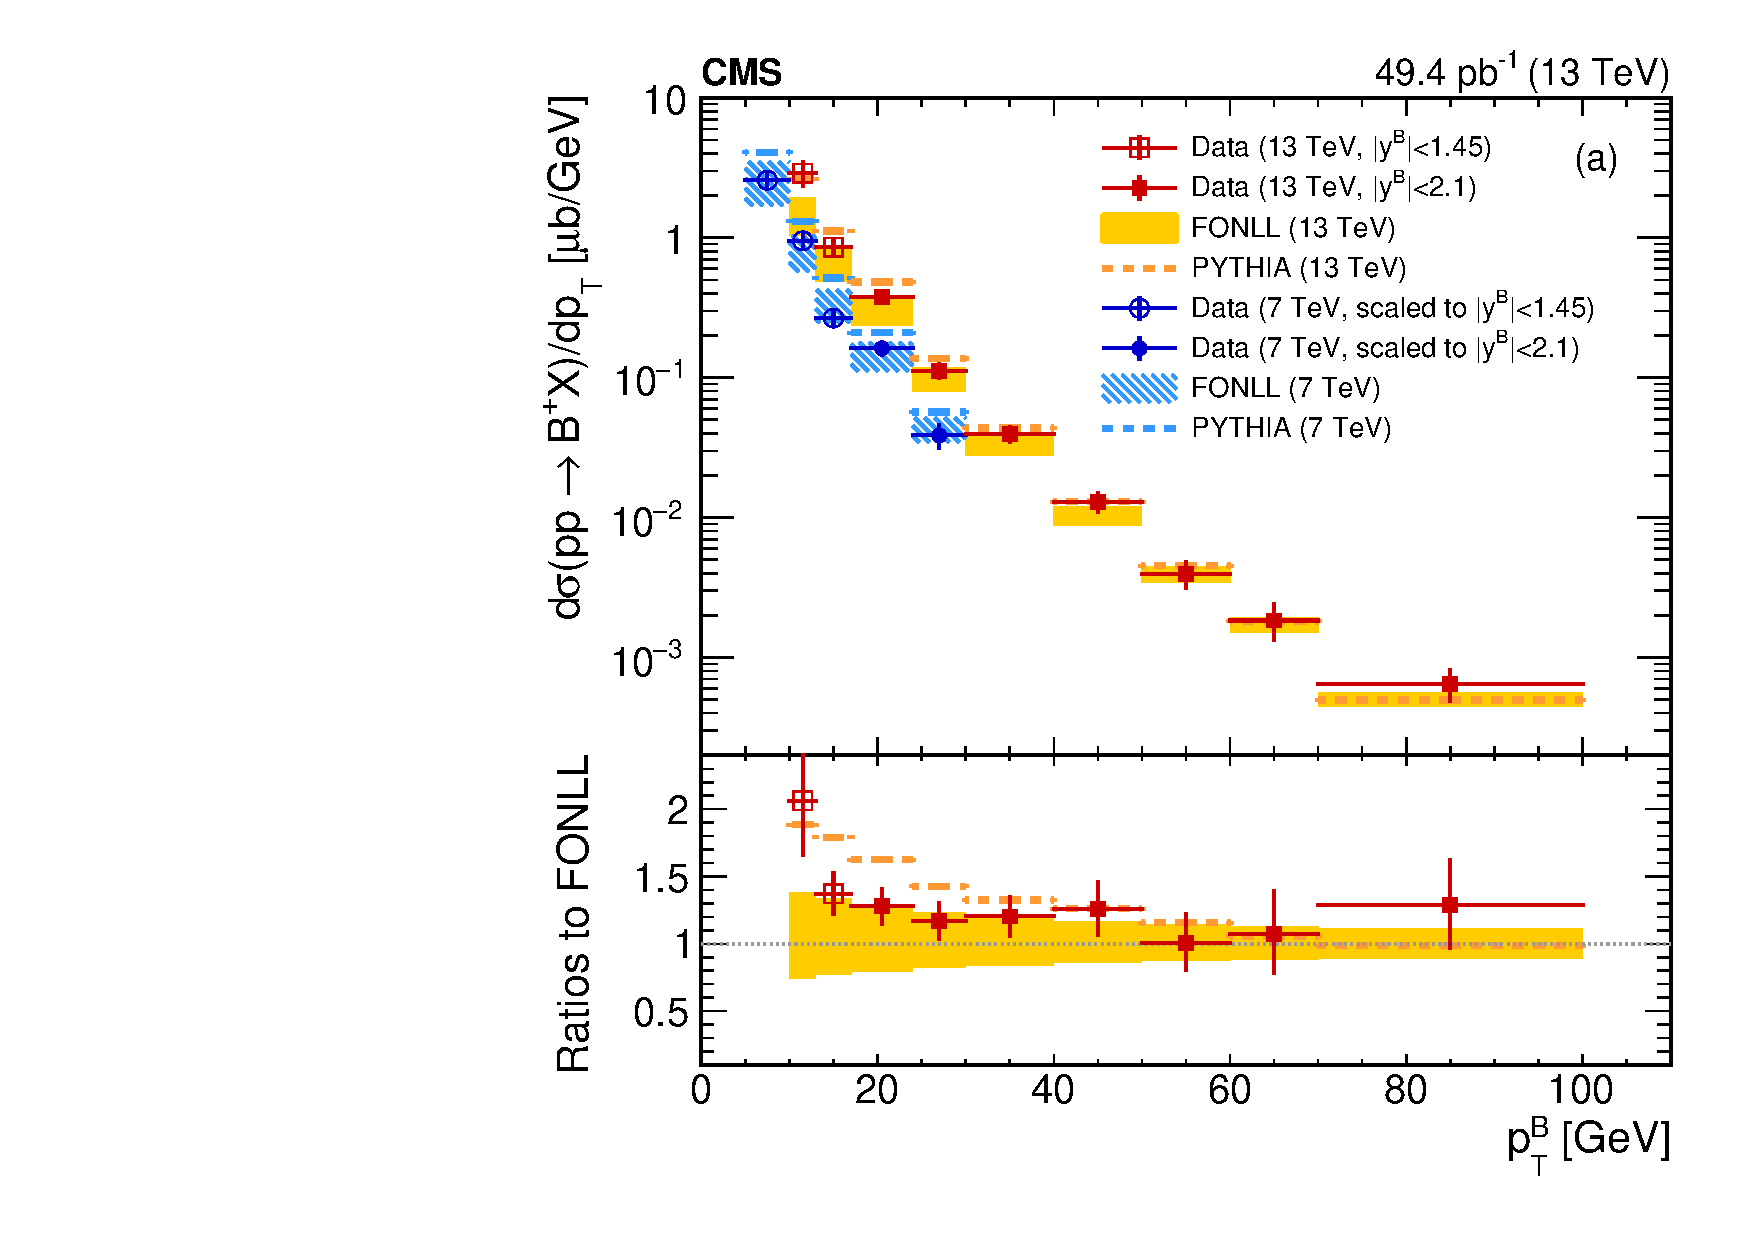
\includegraphics[width=\textwidth]{atlas_bp_production}\\
        $\sigma(\pp \to \Bp X)$ at $\sqrts = \SI{13}{\TeV}$
      \end{center}
    \end{column}
    \begin{column}{0.5\textwidth}
      \begin{center}
        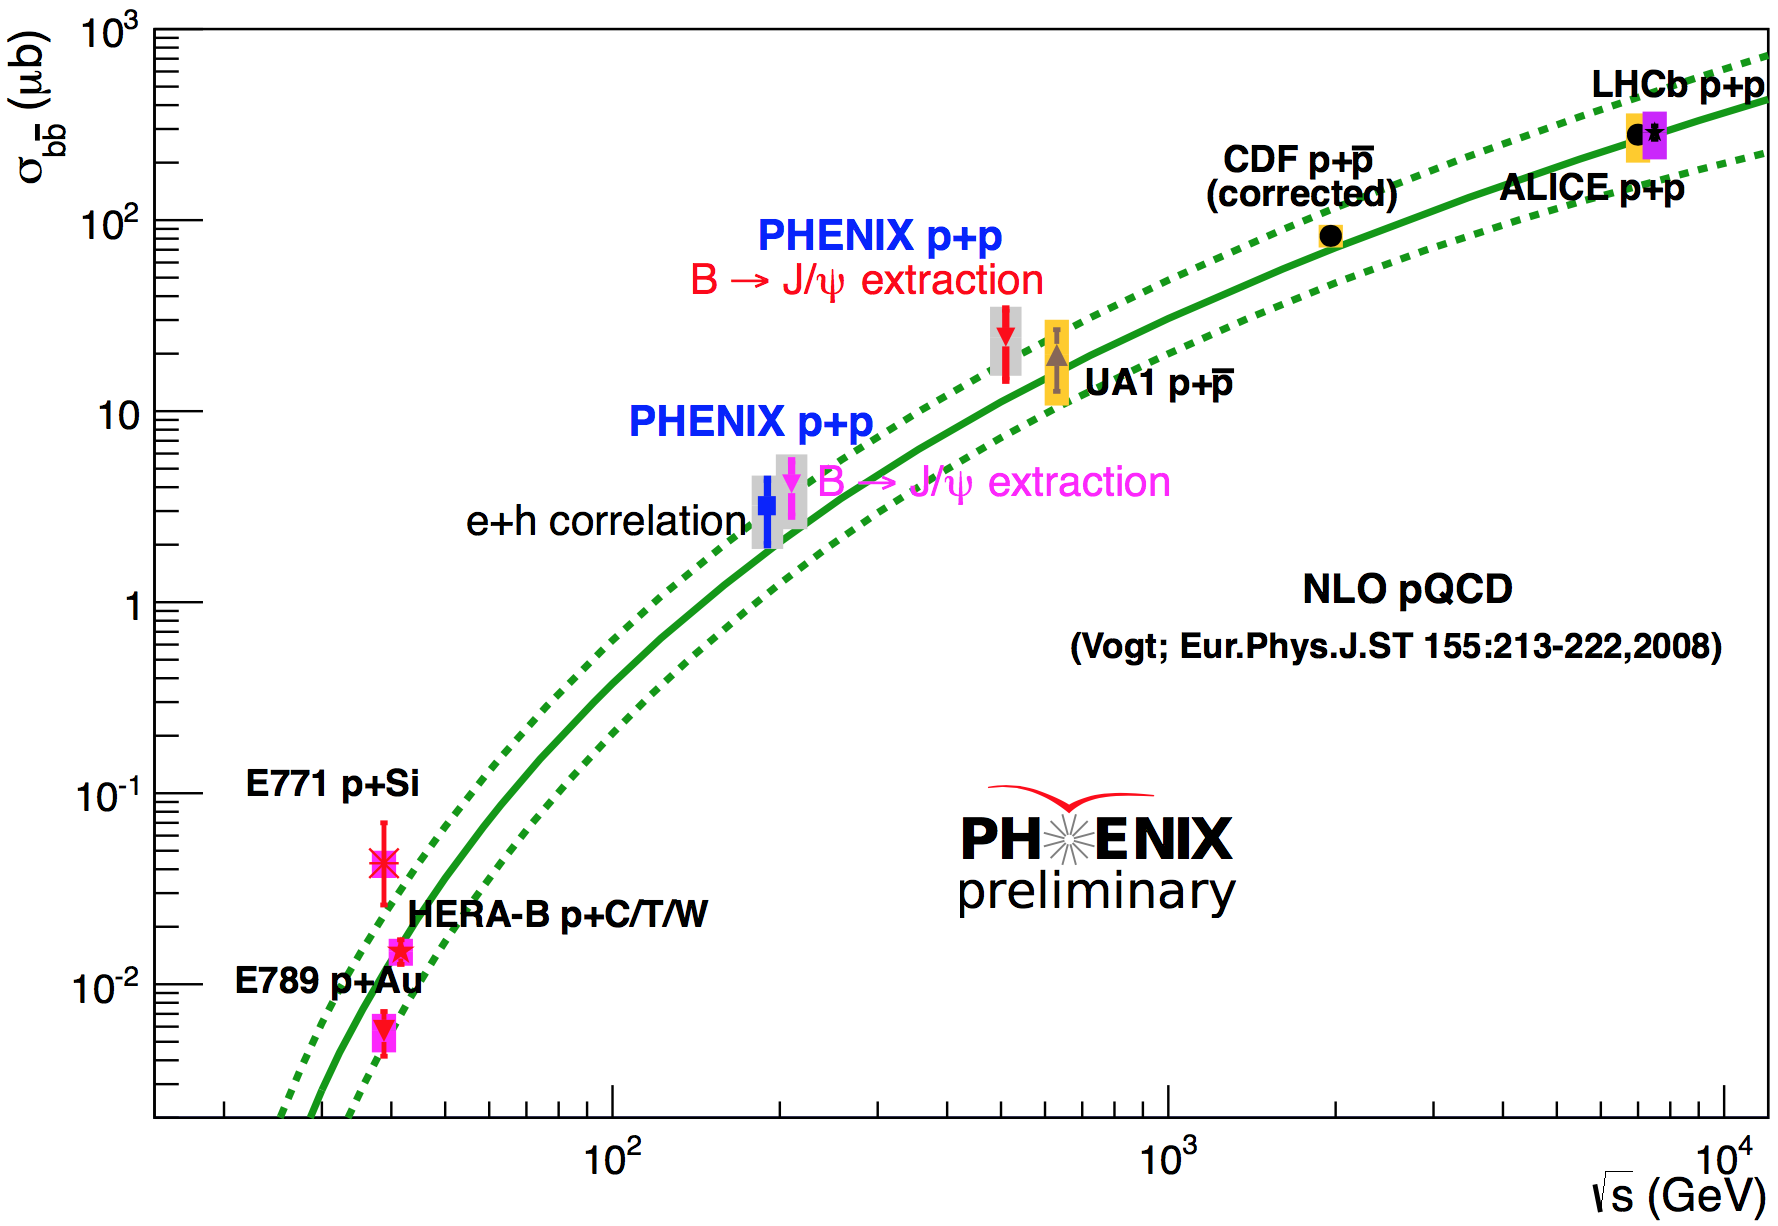
\includegraphics[width=\textwidth]{bbbar_production.png}\\
        New $\sigma(\pp \to \bbbar)$ from PHENIX\\
        at $\sqrts = 200$ and \SI{510}{\GeV}
      \end{center}
    \end{column}
  \end{columns}
\end{frame}

\section{Heavy flavour production in ion collisions}
\begin{frame}{Heavy flavour production in ion collisions%
              \righttitle{\href{https://indico.cern.ch/event/568360/contributions/2471876/}{Z.\ Kang}}}
  Understanding quark-gluon plasma can help in understanding the early universe\par
  \bigskip
  At accelerators, interesting parameter is $R_{H} = \sigma(AA \to H)/\sigma(\pp \to H)$\par
  \bigskip
  % Suitable for highly energetic degrees of freedom interacting via *soft* 
  % radiation
  % Add Glauber gluons to describe dominant effect of transverse momentum 
  % transfer
  % Treat heavy quarks with finite mass terms in the SCET Lagrangian
  Study soft collinear effective theory for describing high \pT\ objects traversing QGP

  \begin{center}
    % Can't model low pT
    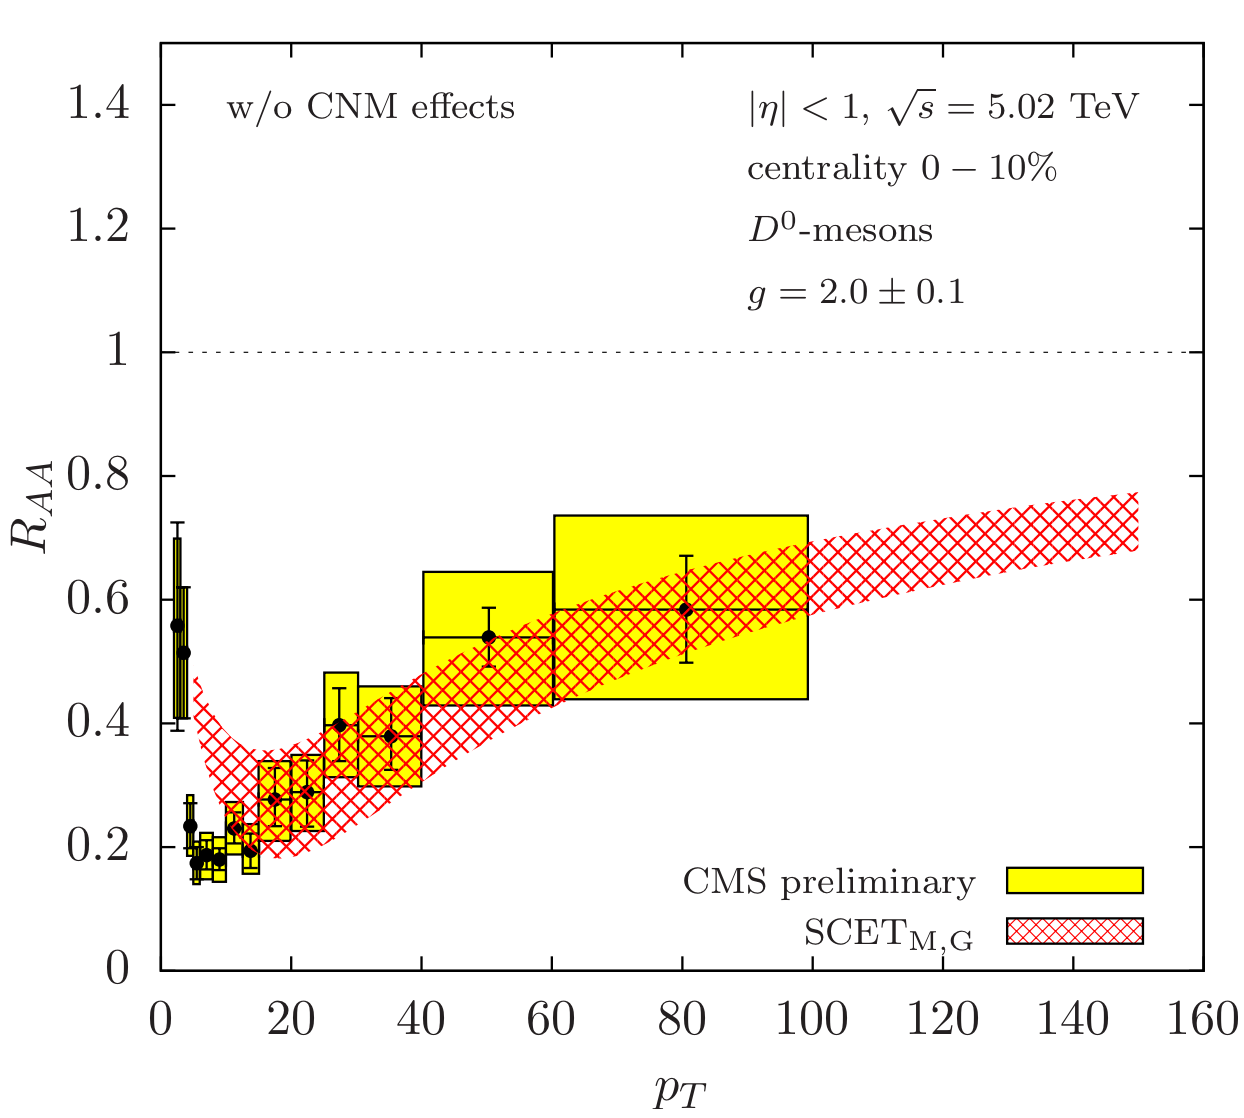
\includegraphics[width=0.5\textwidth]{scet_comparison.png}\\
    New $\sigma(\pp \to \bbbar)$ from PHENIX\\
    at $\sqrts = 200$ and \SI{510}{\GeV}
  \end{center}
\end{frame}

\begin{frame}{Heavy flavour production in ion collisions%
              \righttitle{\href{https://indico.cern.ch/event/568360/contributions/2480993/attachments/1440754/2217961/DIS2017_slides.pdf}{P.\ Rosnet}}}
  Need to disentangle QGP from cold nuclear matter effects\par
  \bigskip
  Use $\proton\text{Pb}$ collisions as a probe of CNM

  \begin{center}
    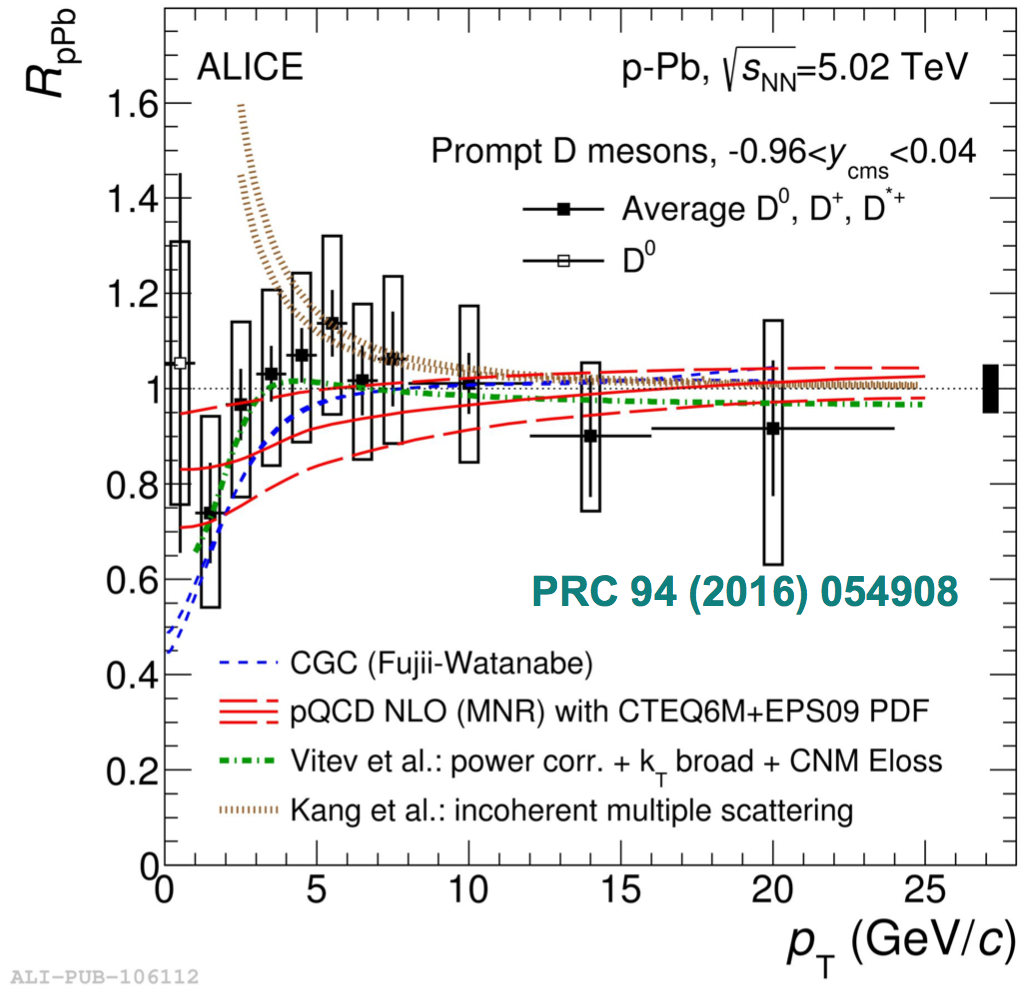
\includegraphics[width=0.5\textwidth]{alice_d0_ppb_production.png}
  \end{center}
\end{frame}

\section{Heavy flavour cross-sections as inputs}
\subsection{Parton density functions}
\begin{frame}{Heavy flavour cross-sections as inputs%
              \righttitle{%
                \href{https://indico.cern.ch/event/568360/contributions/2456401}{J.\ Rojo},
                \href{https://indico.cern.ch/event/568360/contributions/2481104}{S.\ Jones}
              }}{Parton density functions}
  Significant improvement to high and low $x$ models when including (double) differential cross-sections

  \begin{columns}
    \begin{column}{0.5\textwidth}
      \begin{center}
        % Phenomenlogical implications: more accurate predictions for future ep 
        % colliders, constraints on atmospheric prompt neutrino flux
        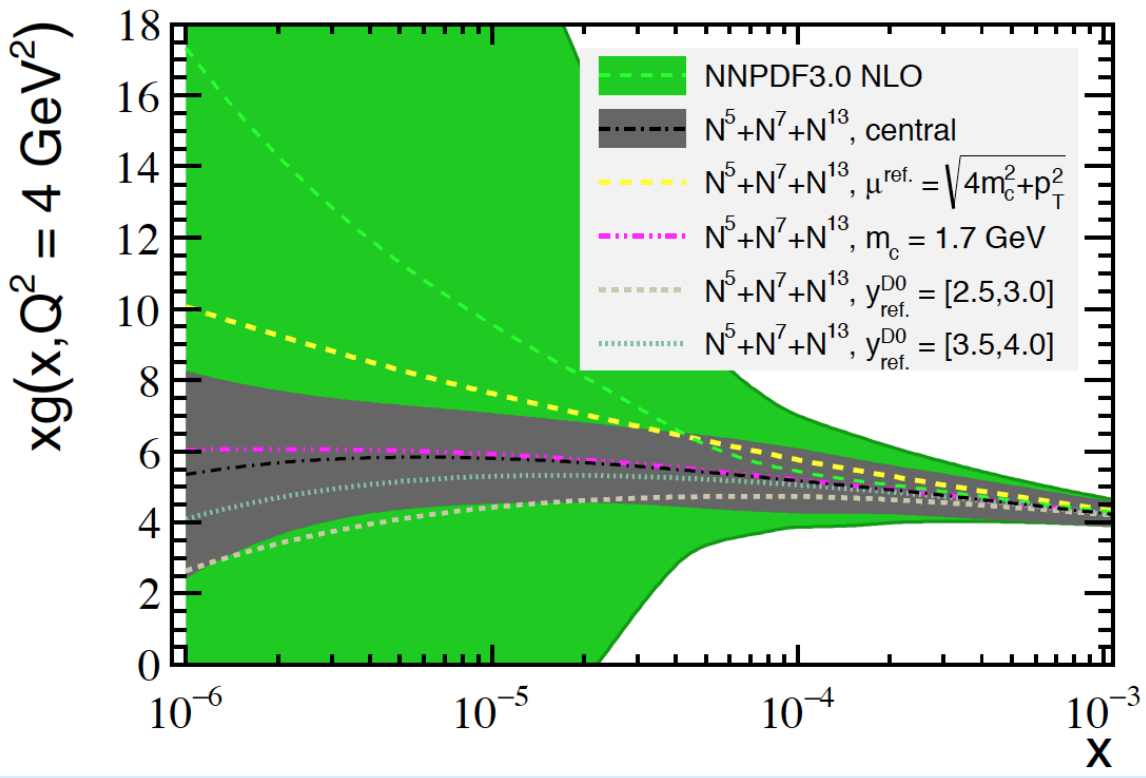
\includegraphics[width=\textwidth]{low_x_pdf_fits.png}\\
        LHCb open charm
      \end{center}
    \end{column}
    \begin{column}{0.5\textwidth}
      \begin{center}
        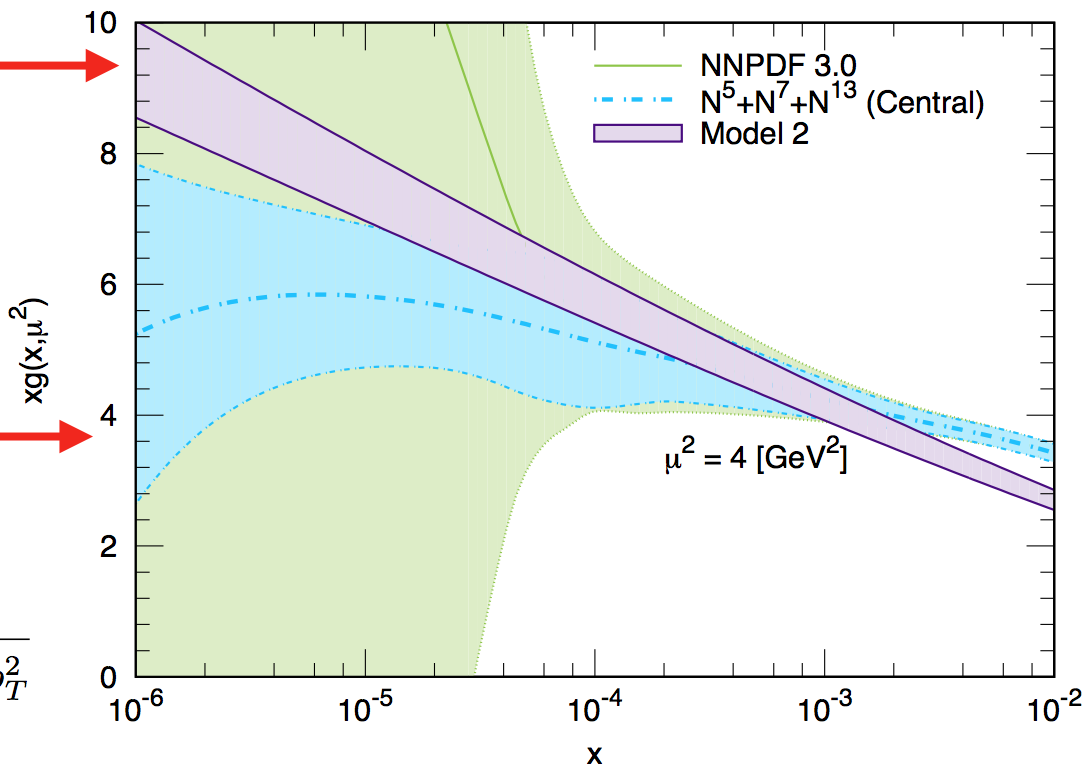
\includegraphics[width=0.95\textwidth]{low_x_pdf_fits_jpsi.png}\\
        LHCb \jpsi{}
      \end{center}
    \end{column}
  \end{columns}
\end{frame}

\begin{frame}{Heavy flavour cross-sections as inputs%
              \righttitle{%
                \href{https://indico.cern.ch/event/568360/contributions/2481101}{E.\ Nocera}
            }}{Parton density functions}
  Significant improvement to high and low $x$ models when including (double) differential cross-sections

  \begin{columns}
    \begin{column}{0.45\textwidth}
      \begin{center}
        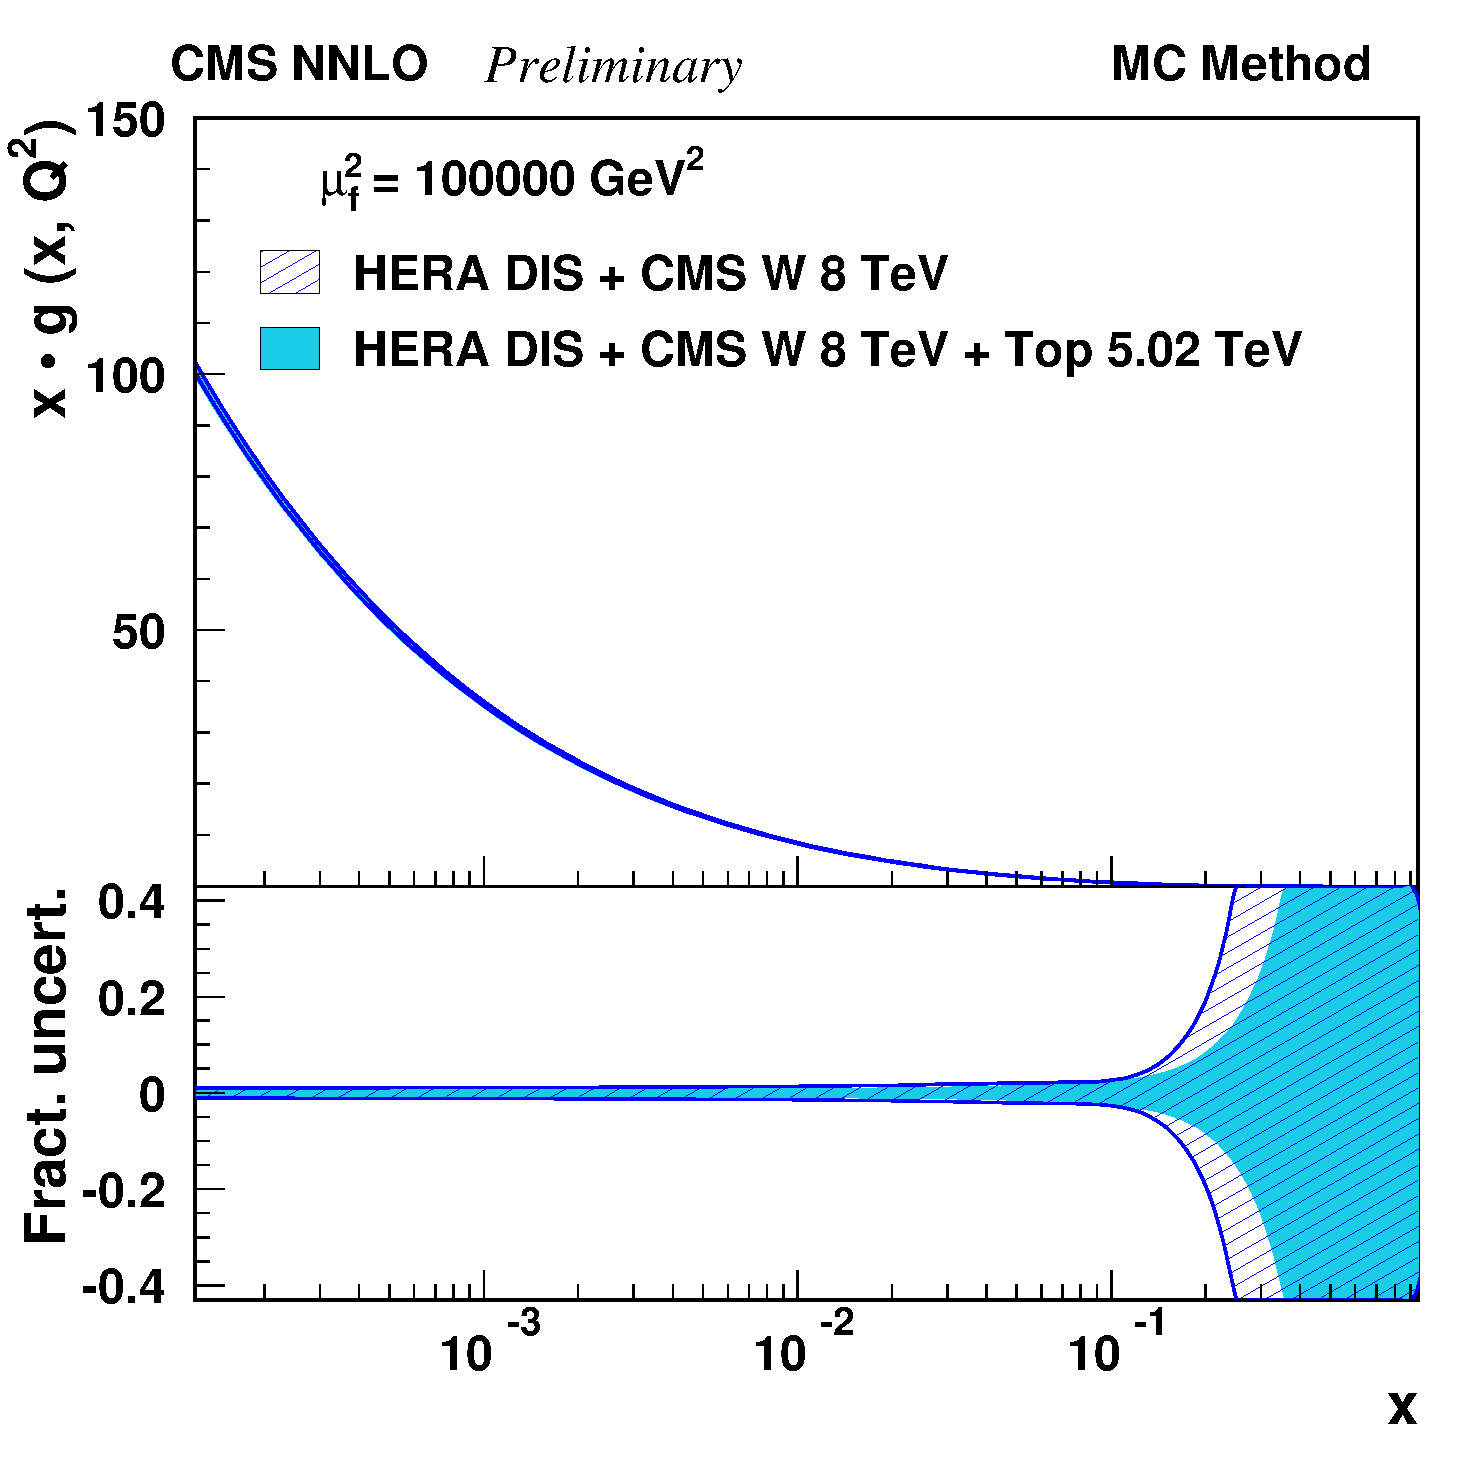
\includegraphics[width=\textwidth]{high_x_pdf_fits_cms}\\
        CMS \ttbar{}
      \end{center}
    \end{column}
    \begin{column}{0.55\textwidth}
      \begin{center}
        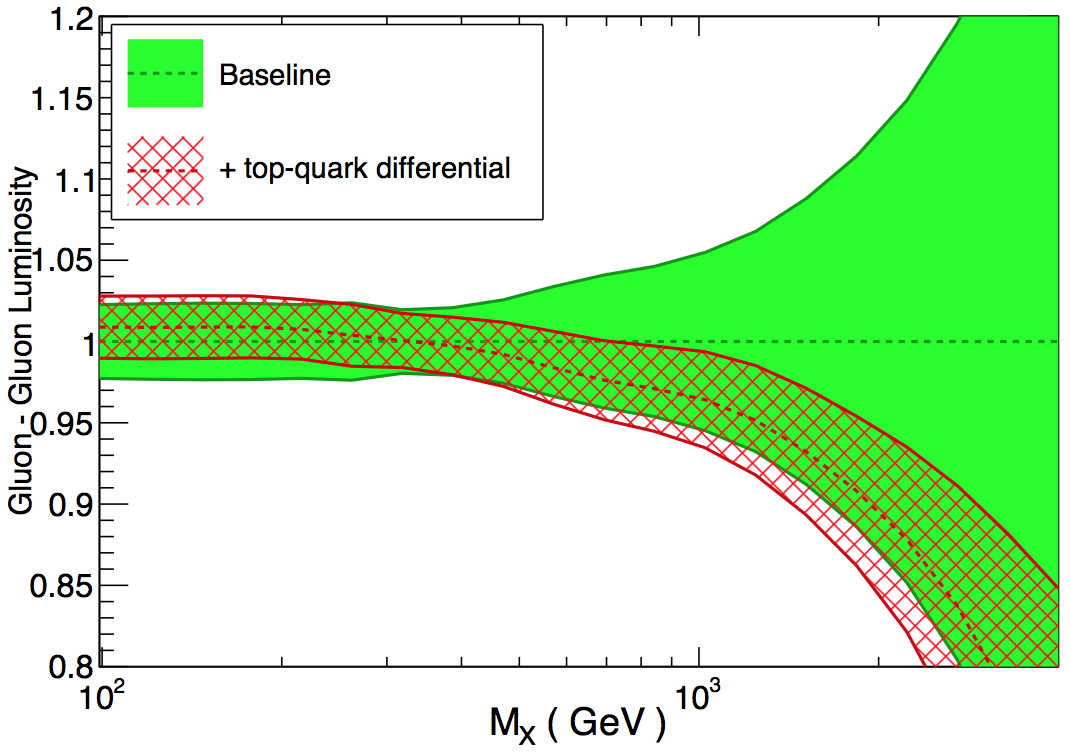
\includegraphics[width=\textwidth]{high_x_pdf_fits.png}\\
        Combined ATLAS and CMS \ttbar{}
      \end{center}
    \end{column}
  \end{columns}
\end{frame}

\subsection{Quark masses}
\begin{frame}{Heavy flavour cross-sections as inputs%
              \righttitle{\href{https://indico.cern.ch/event/568360/contributions/2443302}{G.\ Corcella}}}{Top quark mass}
  Production distributions of top quarks sensitive to $m_{\Ptop}$\par
  \bigskip
  % But: the MC mass includes effects like ISR and FSR and hadronisation, which 
  % affect the 'measured' mass
  Often reported experimentally by varying MC mass and choosing best-fit value to data\par
  \bigskip
  % There are different schemes for defining the mass (pole, MSbar)
  % Generally accepted that there's around a 1–2 GeV difference between the MC 
  % mass and the pole mass
  How to relate MC mass to the `true' mass?

  \begin{center}
    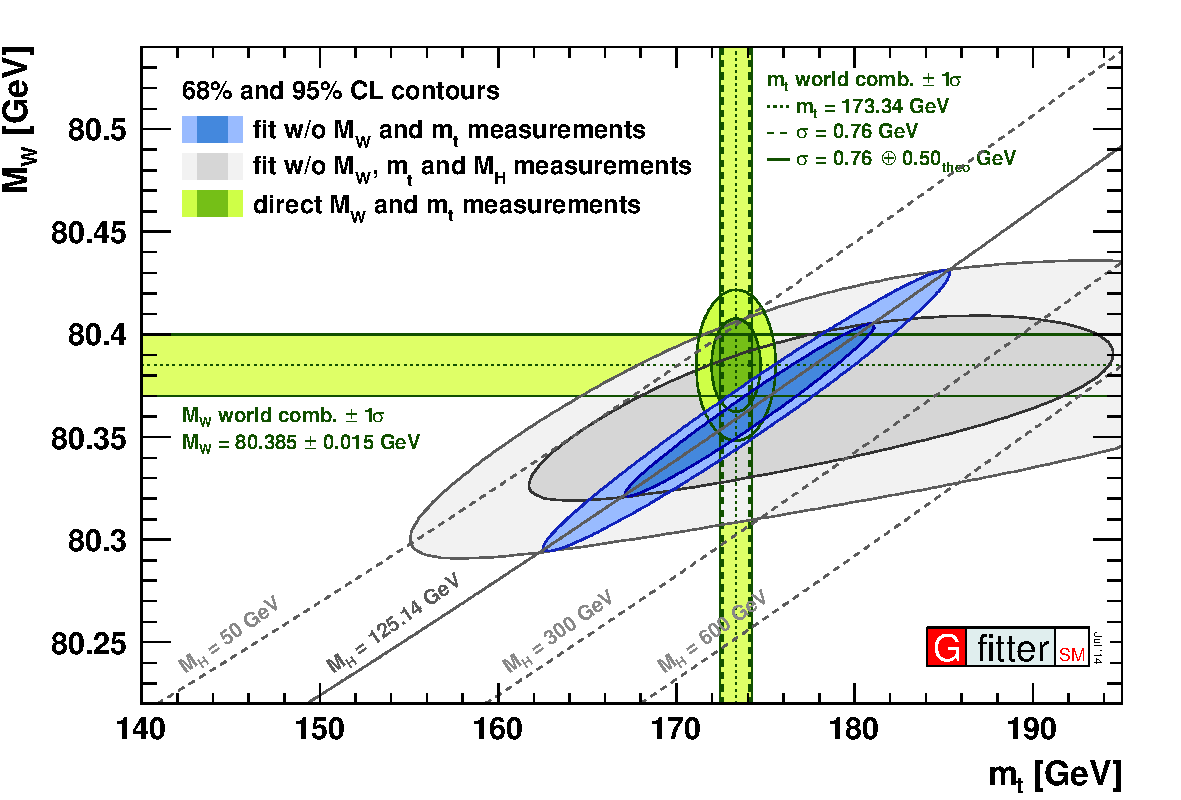
\includegraphics[width=0.5\textwidth]{ew_top_mass_plane}\\
    Top, \PWpm, and Higgs mass relationship very well-defined in the SM
  \end{center}
\end{frame}

\begin{frame}{Heavy flavour cross-sections as inputs%
              \righttitle{\href{https://indico.cern.ch/event/568360/contributions/2480932}{J.\ Kieseler}}}{Top quark mass}
  % Just by shifting the MC mass by +/- 1 GeV
  Usually, include uncertainty on $m_{\Ptop}^{\text{MC}} \leftrightarrow m_{\Ptop}^{\text{true}}$ relation as uncertainty on $\sigma(\ttbar)$\par
  \bigskip
  % Mass gives shape differences, xsec gives normalisation
  Alternative: simultaneously fit for $\sigma(\ttbar)$ and $m_{\Ptop}^{\text{MC}}$, determine $\text{MC} \leftrightarrow \text{true}$ relationship later

  \begin{columns}
    \begin{column}{0.5\textwidth}
      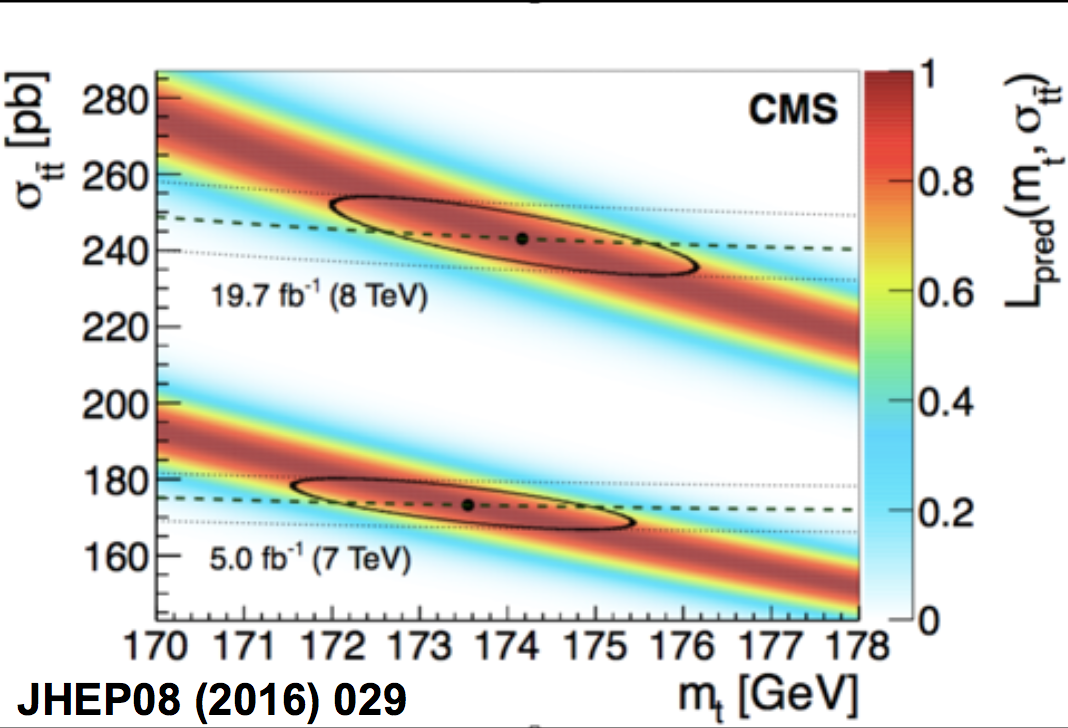
\includegraphics[width=\textwidth]{top_mass_mc_dependent}
    \end{column}
    \begin{column}{0.5\textwidth}
      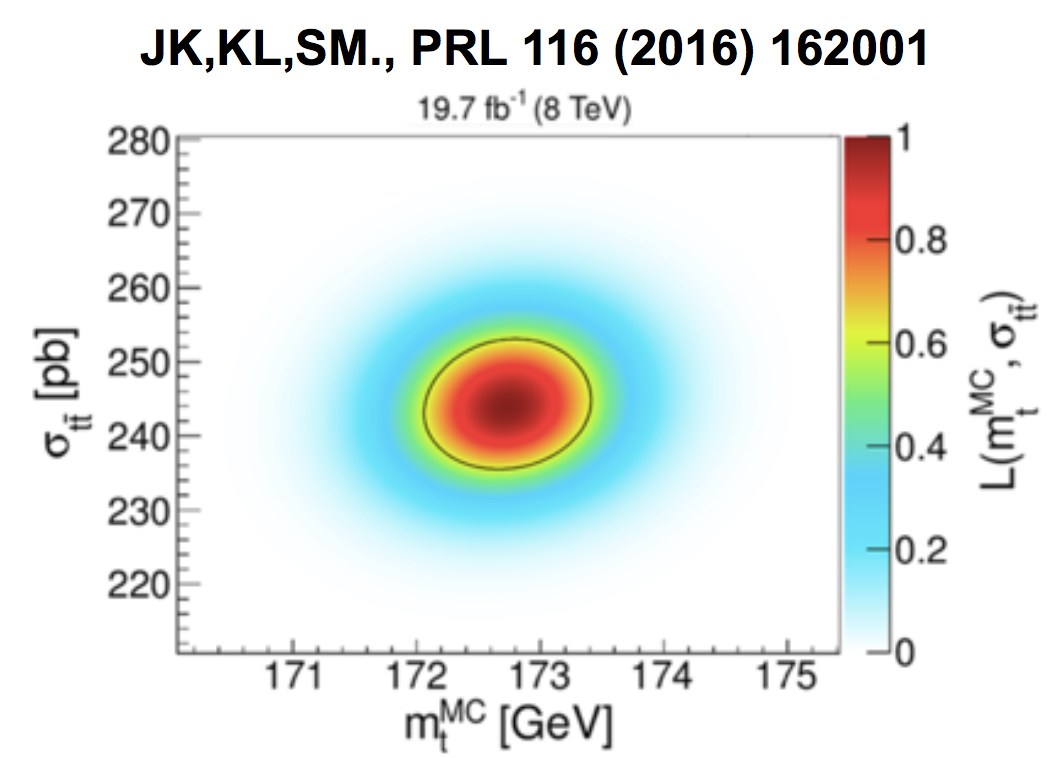
\includegraphics[width=\textwidth]{top_mass_mc_independent}
    \end{column}
  \end{columns}
\end{frame}

\begin{frame}{Heavy flavour cross-sections as inputs%
              \righttitle{\href{https://indico.cern.ch/event/568360/contributions/2471878}{A.\ Geiser}}}{Charm and bottom quark masses}
    \begin{columns}
      \begin{column}{0.5\textwidth}
        Can measure the running of \Pcharm\ and \Pbottom\ using DIS data\par
        \bigskip
        \structure{Interpretation}: higher scales $\leftrightarrow$ smaller distances, see less gluon field around the quark, hence less energy
      \end{column}
      \begin{column}{0.5\textwidth}
        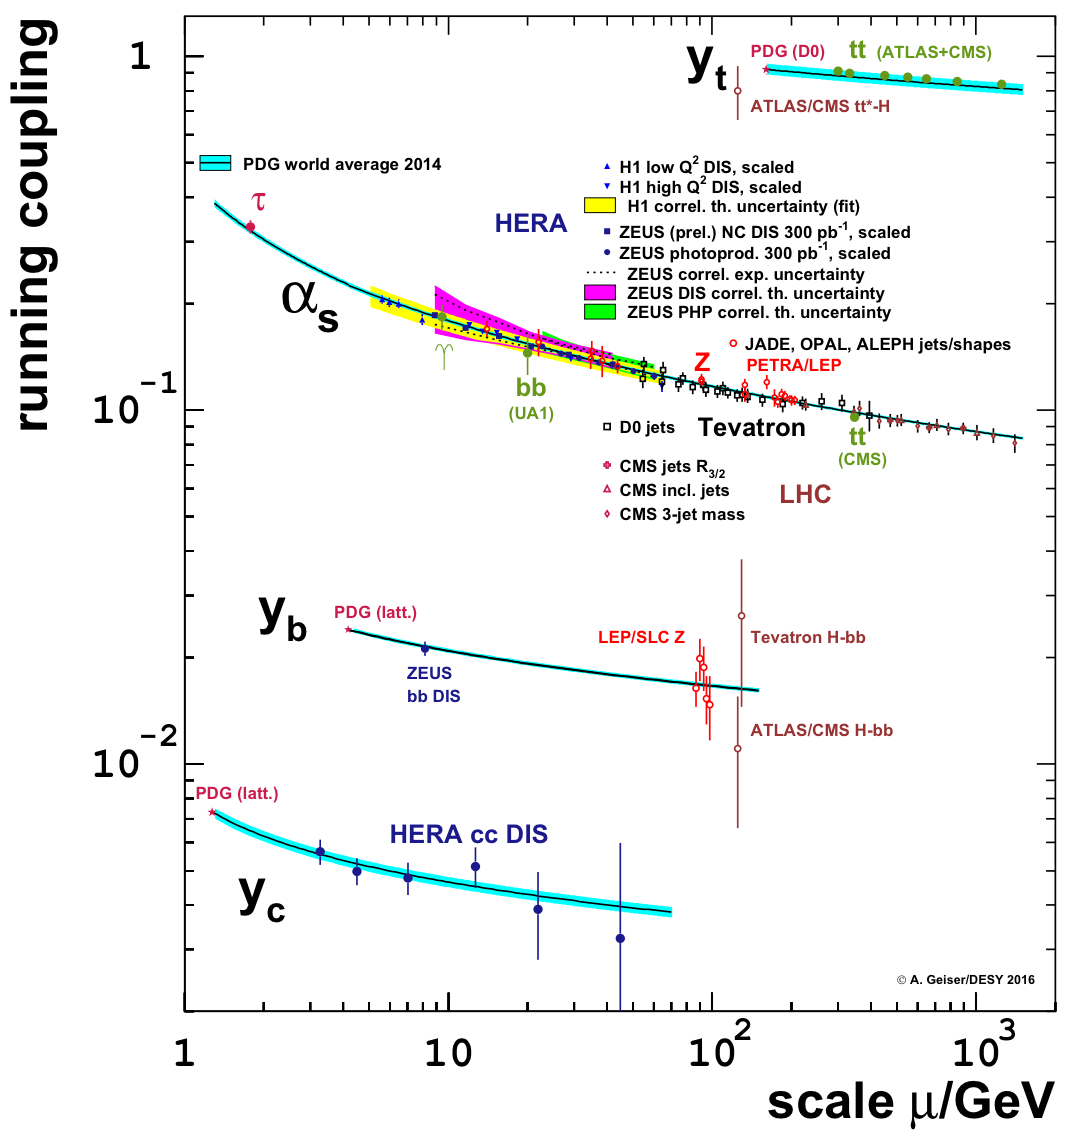
\includegraphics[width=\textwidth]{constant_running.png}
      \end{column}
    \end{columns}
\end{frame}

% \begin{frame}{Heavy flavour cross-sections as inputs%
%               \righttitle{%
%                 \href{https://indico.cern.ch/event/568360/contributions/2473542/}{N-A.\ Rosien},
%                 \href{https://indico.cern.ch/event/568360/contributions/2435613/}{P.\ David}
%               }}{\CP\ violation with top production},
% \end{frame}

\section{Properties of \texorpdfstring{\B}{B} and \texorpdfstring{\D}{D} hadrons}
\begin{frame}{Charm and beauty hadron properties}
  Heavy flavour hadron decays encompass a rich phenomenology:
  \begin{itemize}
    \item Neutral meson mixing, e.g.\ $\Dz \leftrightarrow \Dzbar$
    \item Violation of \CP\ symmetry via the CKM matrix
    % Complementary to direct searches, sensitive to higher scales
    \item Sensitive to new particles entering loops in decay diagrams
  \end{itemize}
  \bigskip
  Recent tensions in lepton universality and flavour-changing neutral currents (FCNC)\par
  \bigskip
  Several experiments competing, from no-longer-running to starting up this year
\end{frame}

\begin{frame}{Charm and beauty hadron properties%
              \righttitle{\href{https://indico.cern.ch/event/568360/contributions/2471872}{X.\ Shi}}}
  \begin{columns}
    \begin{column}{0.5\textwidth}
      \begin{center}
        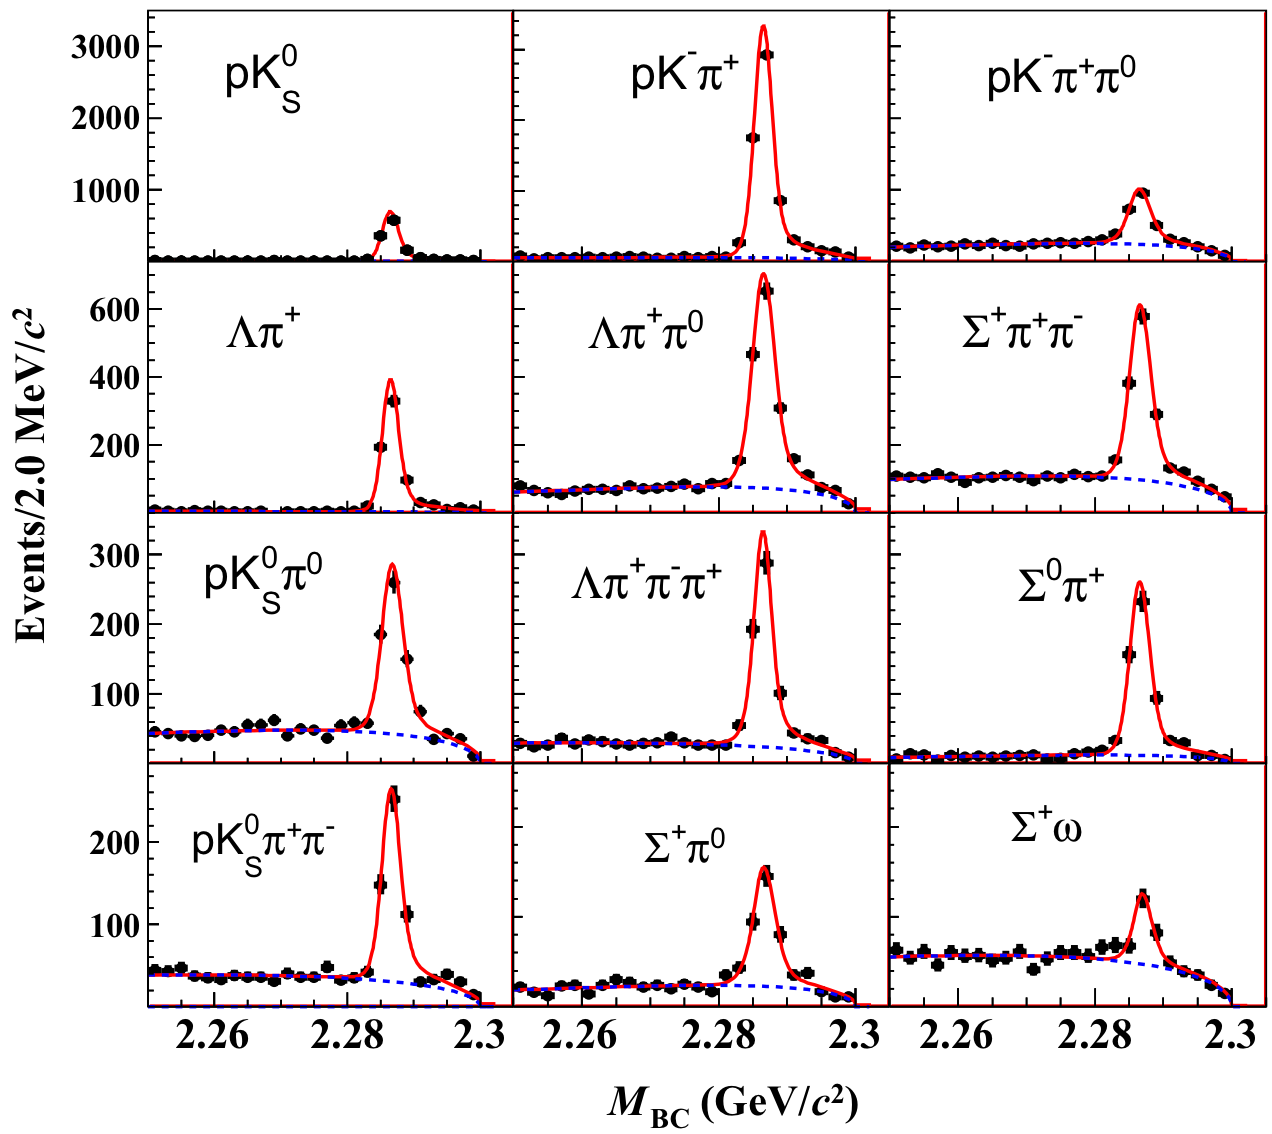
\includegraphics[width=\textwidth]{lc_yields.png}
      \end{center}
    \end{column}
    \begin{column}{0.5\textwidth}
      Large set of results from BESIII\par
      \bigskip
      Significant reduction in branching fraction uncertainties\par
      \bigskip
      % Has been a limiting factor in measurements such as V_ub
      \structure{Example}: $\mathcal{B}(\Lcp \to \proton\Km\pip)$ from \SI{25}{\percent} relative uncertainty (PDG) to \SI{6}{\percent}
    \end{column}
  \end{columns}
\end{frame}

\begin{frame}{Charm and beauty hadron properties%
              \righttitle{\href{https://indico.cern.ch/event/568360/contributions/2497347/}{L.\ Pescatore}}}
  % First observation after combination with CMS
  % There are FCNC results from ATLAS and CMS that I'm skipping!
  First observation by a single experiment of the FCNC process $\Bs \to \mup\mum$
  \bigskip

  \begin{columns}
    \begin{column}{0.5\textwidth}
      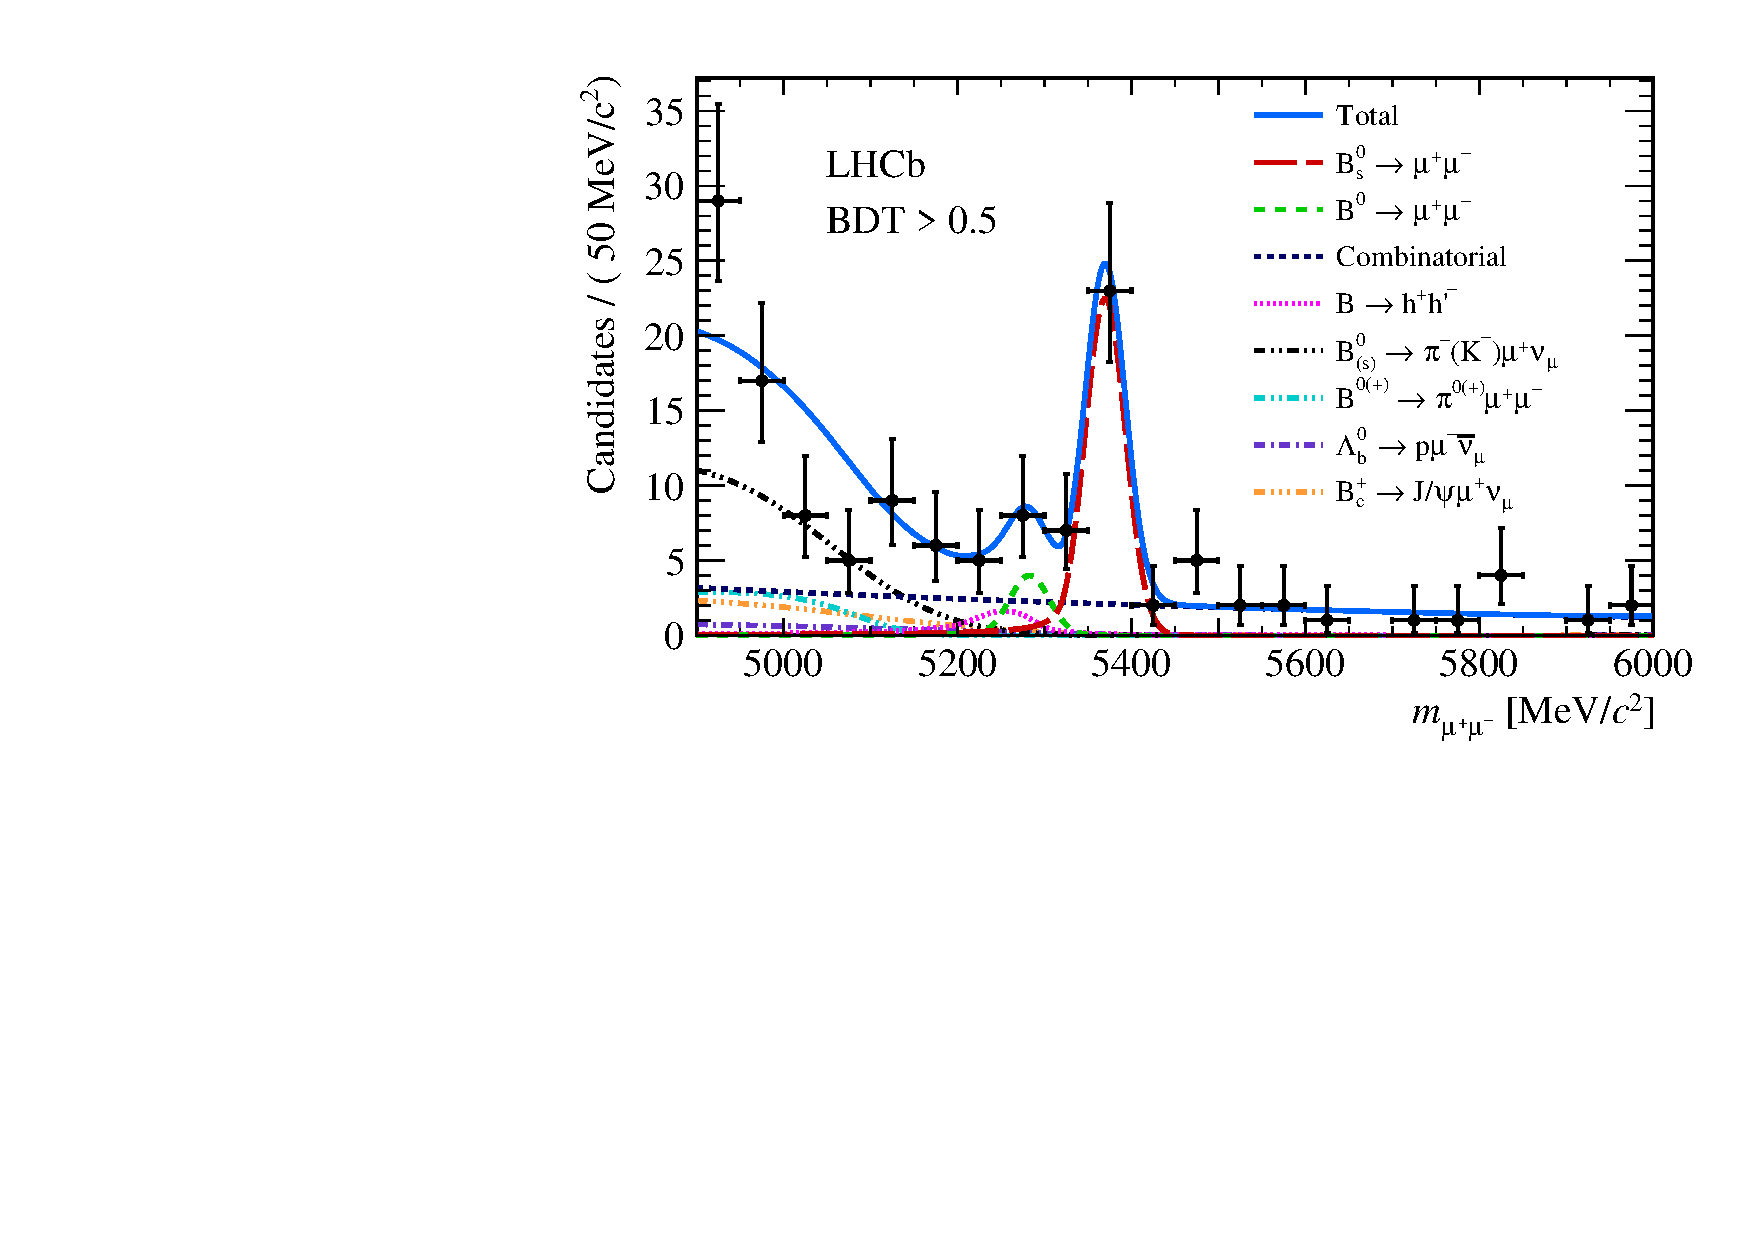
\includegraphics[width=\textwidth]{bstomumu_fit}
    \end{column}
    \begin{column}{0.5\textwidth}
      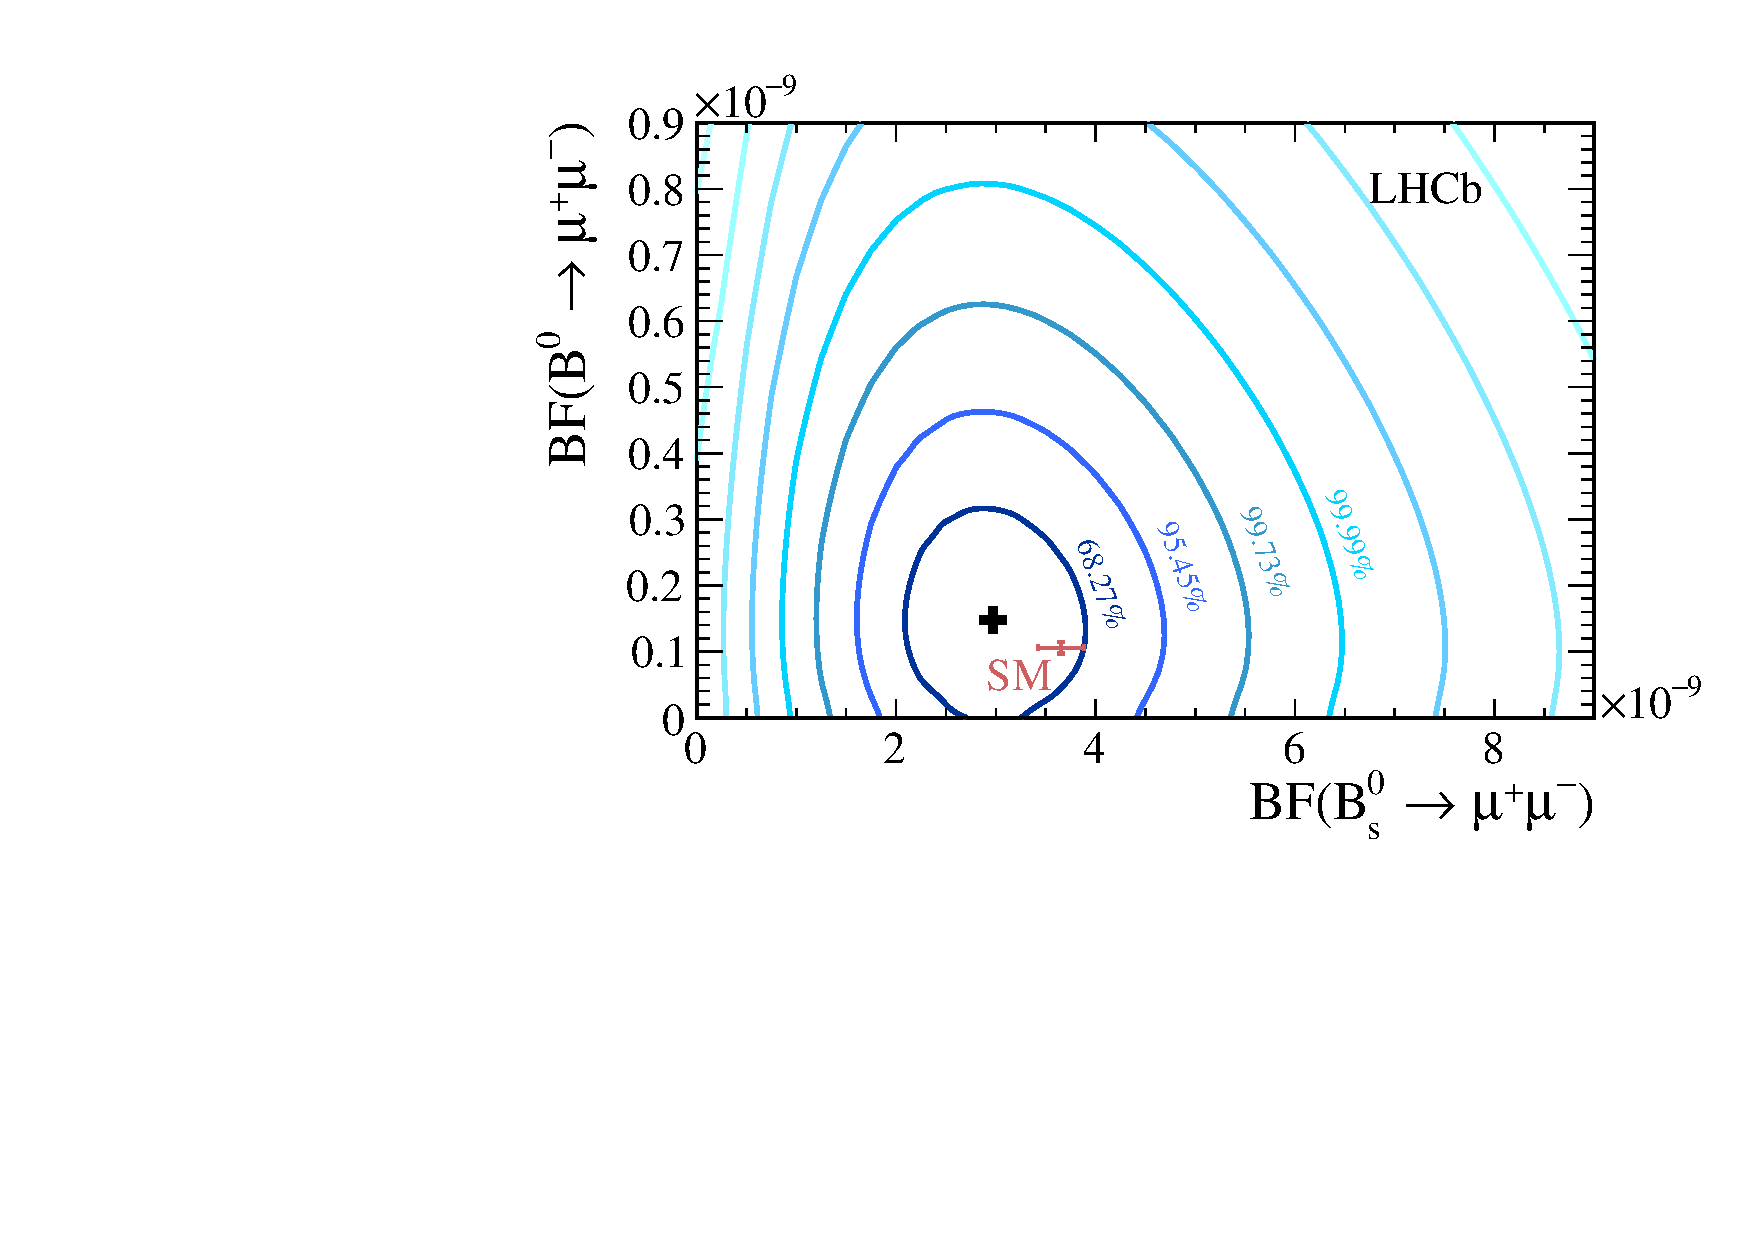
\includegraphics[width=\textwidth]{bstomumu_sm}
    \end{column}
  \end{columns}
  \vspace{-0.5cm}
  \begin{center}
    \[
      \mathcal{B}(\Bs \to \mup\mum) = (2.8 \pm 0.9) \times 10^{-9} \quad (\SI{7.8}{\sigma})
    \]
    \[
      \mathcal{B}(\Bz \to \mup\mum) = (1.6^{+1.1}_{-0.9}) \times 10^{-10} \quad (\SI{1.9}{\sigma})
    \]
  \end{center}
\end{frame}

\begin{frame}{Charm and beauty hadron properties%
  \righttitle{\href{https://indico.cern.ch/event/568360/contributions/2471874/}{P.\ Chang}}}{Anomalies}
  \begin{columns}
    \begin{column}{0.5\textwidth}
      \[
        R(\Dst) = \frac{%
          \mathcal{B}(\decay{\B}{D^{(*)}\Ptau^{-}\APnut})
          }{%
          \mathcal{B}(\decay{\B}{D^{(*)}\mum\APnum})
        }
      \]
      Test lepton universality\par
      \bigskip
      Sensitive to NP models like charged Higgs\par
      \bigskip
      Precise SM prediction due to cancellation of hadronic effects
    \end{column}
    \begin{column}{0.5\textwidth}
      \begin{center}
        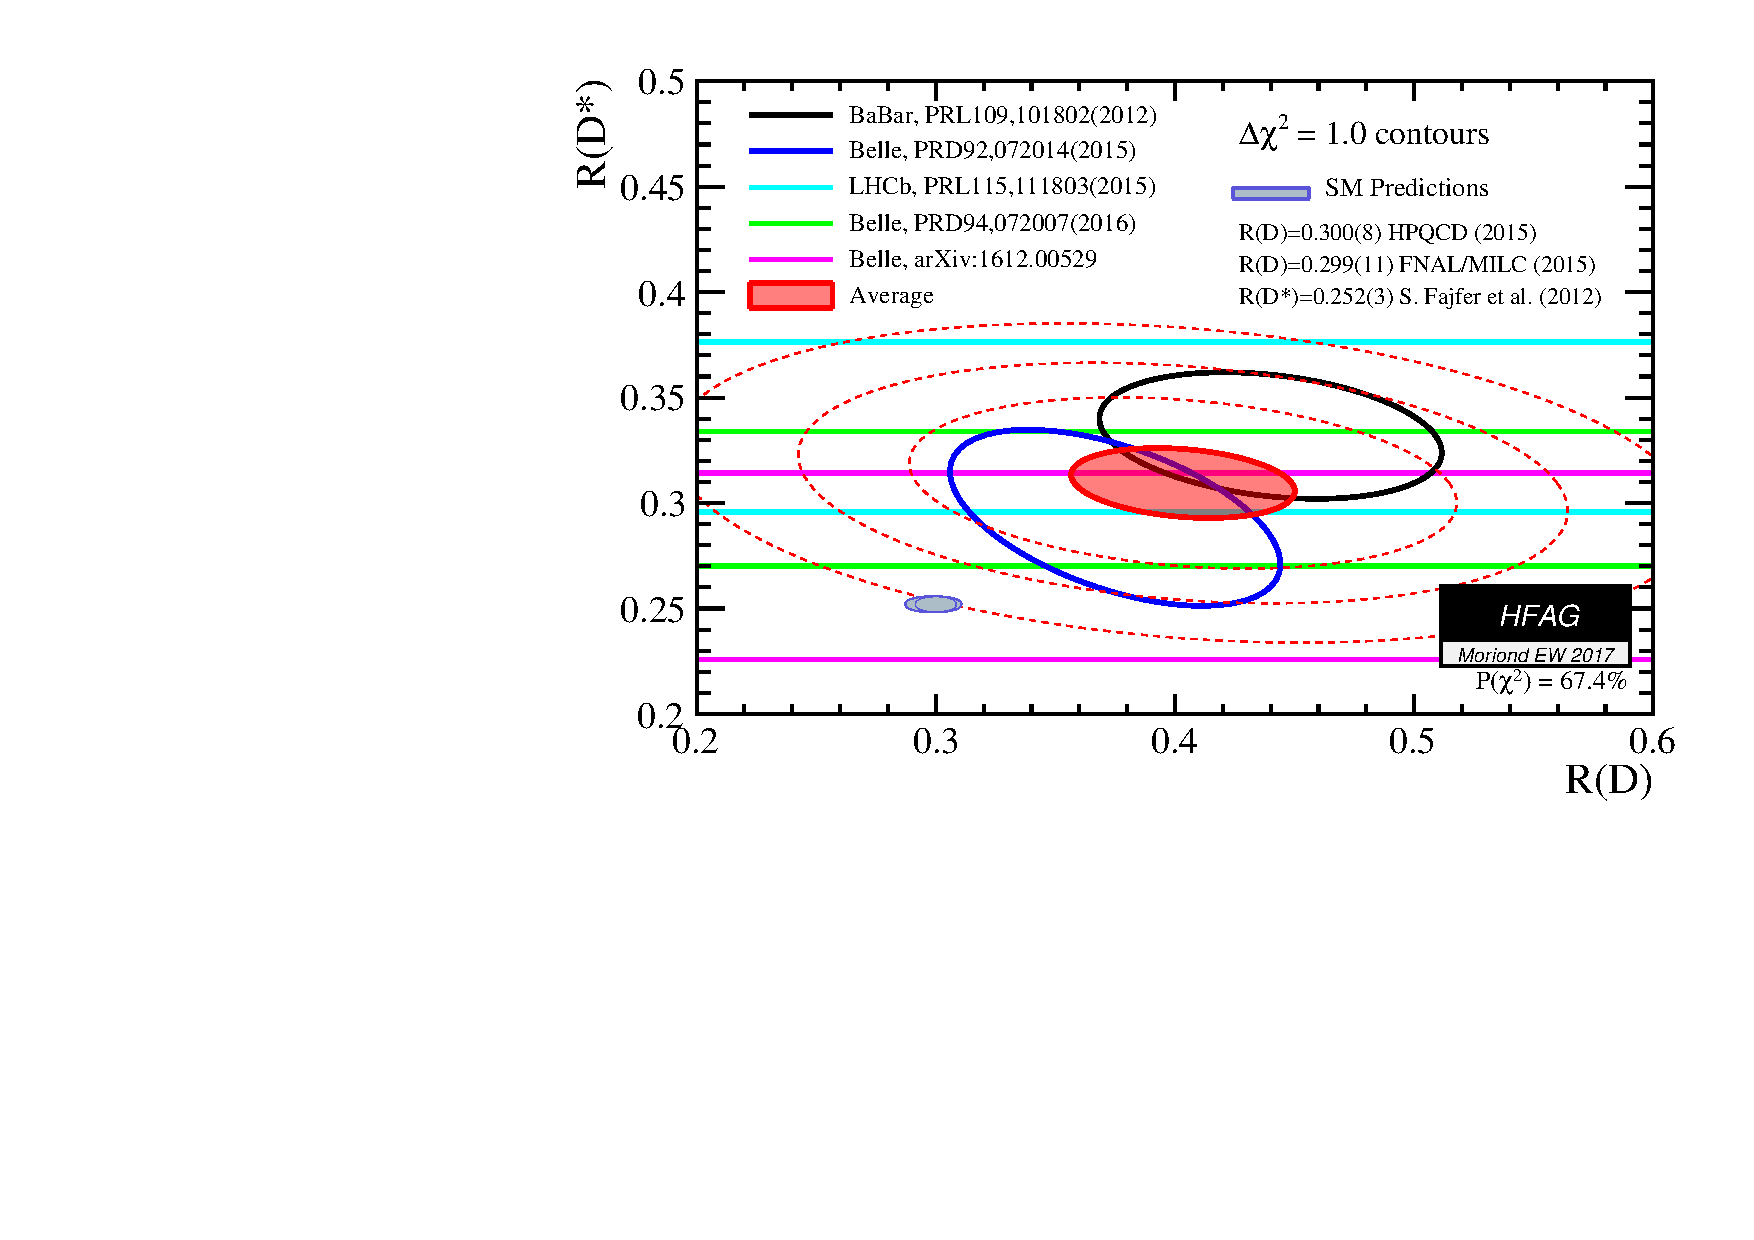
\includegraphics[width=\textwidth]{rdrds_winter2017}\\
        % Belle result's nice because it uses a hadronic tau reconstruction
        % Need a little more data: Belle 2 and LHCb Run 2
        \structure{New} Belle result consistent with SM,\\
        but still a \SI{4}{\sigma} tension
      \end{center}
    \end{column}
  \end{columns}
\end{frame}

\begin{frame}{Charm and beauty hadron properties%
              \righttitle{%
                \href{https://indico.cern.ch/event/568360/contributions/2471874/}{P.\ Chang},
                \href{https://indico.cern.ch/event/568360/contributions/2497347/}{L.\ Pescatore}}}{Anomalies}
  Experimental data exceeds predictions for effective operator $P_{5}'$ in $\decay{B}{K^{*}\mum\mup}$\par
  \bigskip
  If significant, would require non-SM-like change in vector coupling strength $\mathcal{C}_{9}$\par
  \bigskip
  New results from Belle in both electron and muon modes and multiple $K^{*}$ states
  \begin{center}
    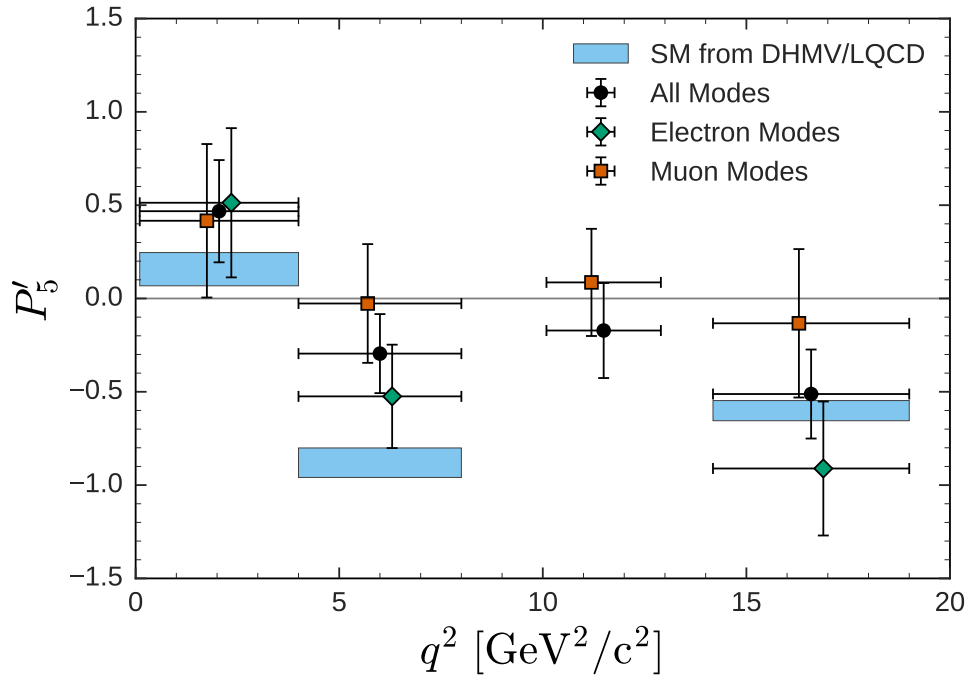
\includegraphics[width=0.5\textwidth]{p5prime.png}\\
    No lepton universality breaking, but \SI{2.5}{\sigma} deviation in one $P_{5}'$ bin
  \end{center}
\end{frame}

\section{Exotic hadrons}
\begin{frame}{Exotic hadrons%
              \righttitle{\href{https://indico.cern.ch/event/568360/contributions/2471891/}{U.\ Tamponi}}}
  % `Exotics' are bound states of 4 or more quarks\par
  % \bigskip
  % Could be bound as tetra/pentaquarks, or as molecules, a rescattering effect\ldots\par
  % \bigskip
  % Significant effort not just finding new states, but characterising their transitions
  \bigskip
  \begin{columns}
    \begin{column}{0.5\textwidth}
      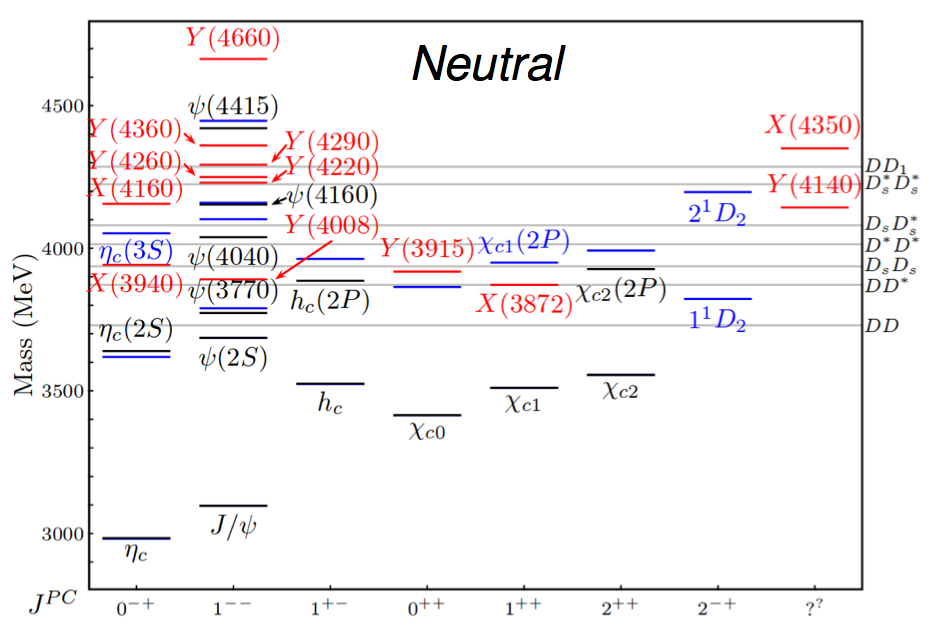
\includegraphics[width=\textwidth]{exotic_spectrum.png}
    \end{column}
    \begin{column}{0.5\textwidth}
      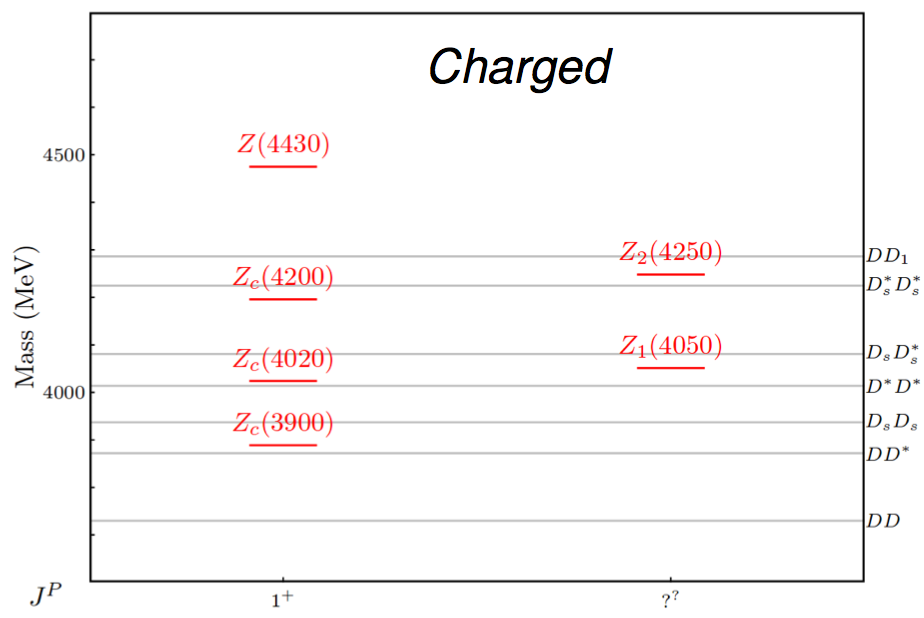
\includegraphics[width=\textwidth]{exotic_spectrum_charged.png}
    \end{column}
  \end{columns}
  \begin{center}
    Expansive set of known exotic states so far
  \end{center}
\end{frame}

\section{Exotic hadrons}
\begin{frame}{Exotic hadrons%
              \righttitle{%
                \href{https://indico.cern.ch/event/568360/contributions/2471891/}{U.\ Tamponi},
                \href{https://indico.cern.ch/event/568360/contributions/2471897/}{M.\ Kavatsyuk}
              }}
  Systematic study of states presented by Belle and BESIII
  \bigskip
  \begin{columns}
    \begin{column}{0.5\textwidth}
      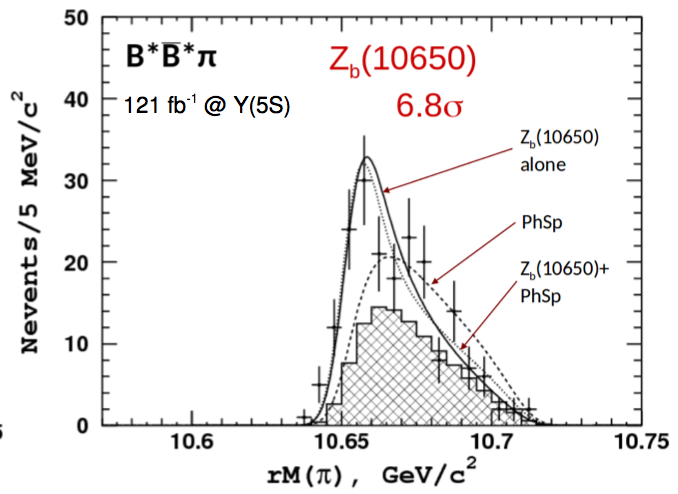
\includegraphics[width=0.9\textwidth]{z10650_belle.png}
    \end{column}
    \begin{column}{0.5\textwidth}
      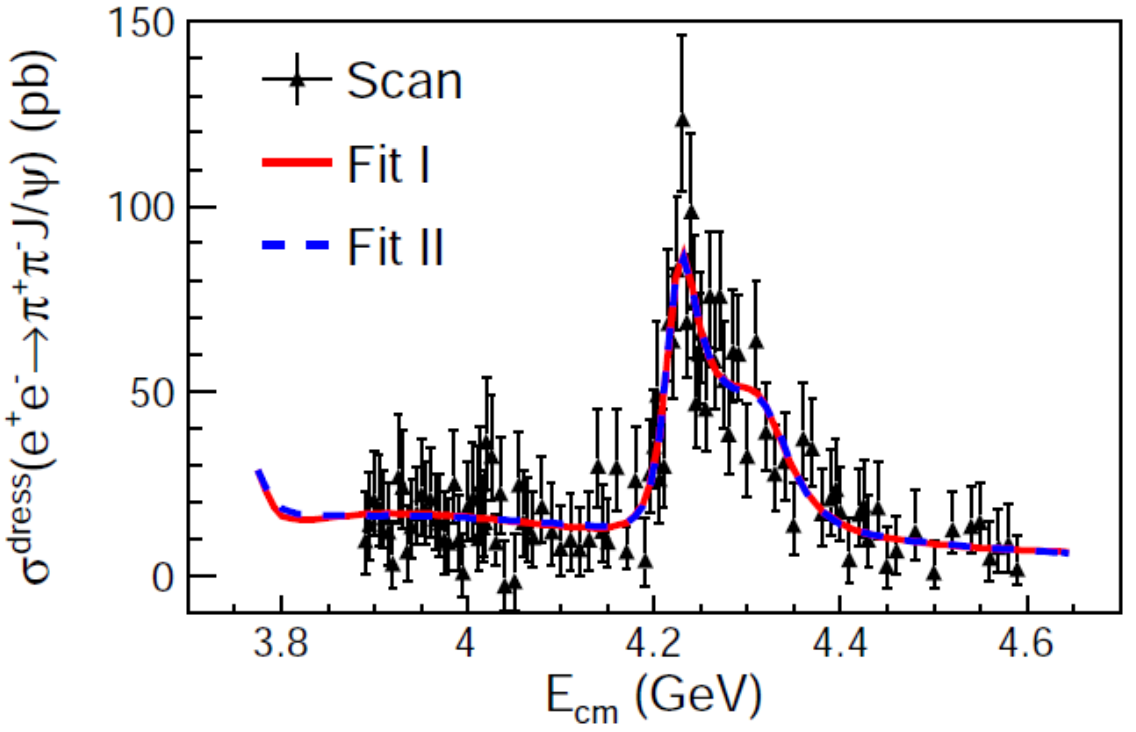
\includegraphics[width=\textwidth]{exotics_scan_besiii.png}
    \end{column}
  \end{columns}
  \bigskip
  Further experimental and theoretical study of currently-known states is \structure{crucial}
\end{frame}

\begin{frame}{Exotic hadrons%
              \righttitle{%
                \href{https://indico.cern.ch/event/568360/contributions/2481015/}{I.\ Bertram},
                \href{https://indico.cern.ch/event/568360/contributions/2471944/}{P.\ Ronchese}
              }}
  D\O\ collaboration announced discovery of $X(5568)$ state found in $\Bs\pip$ spectrum\par
  \bigskip
  % 3.2 sigma
  First used $\decay{\Bs}{\jpsi\phi}$ decays, now report a consistent structure using $\decay{\Bs}{\Dsp\mum X}$\par
  \bigskip
  LHCb nor CMS have been able to confirm the observation
  \begin{columns}
    \begin{column}{0.5\textwidth}
      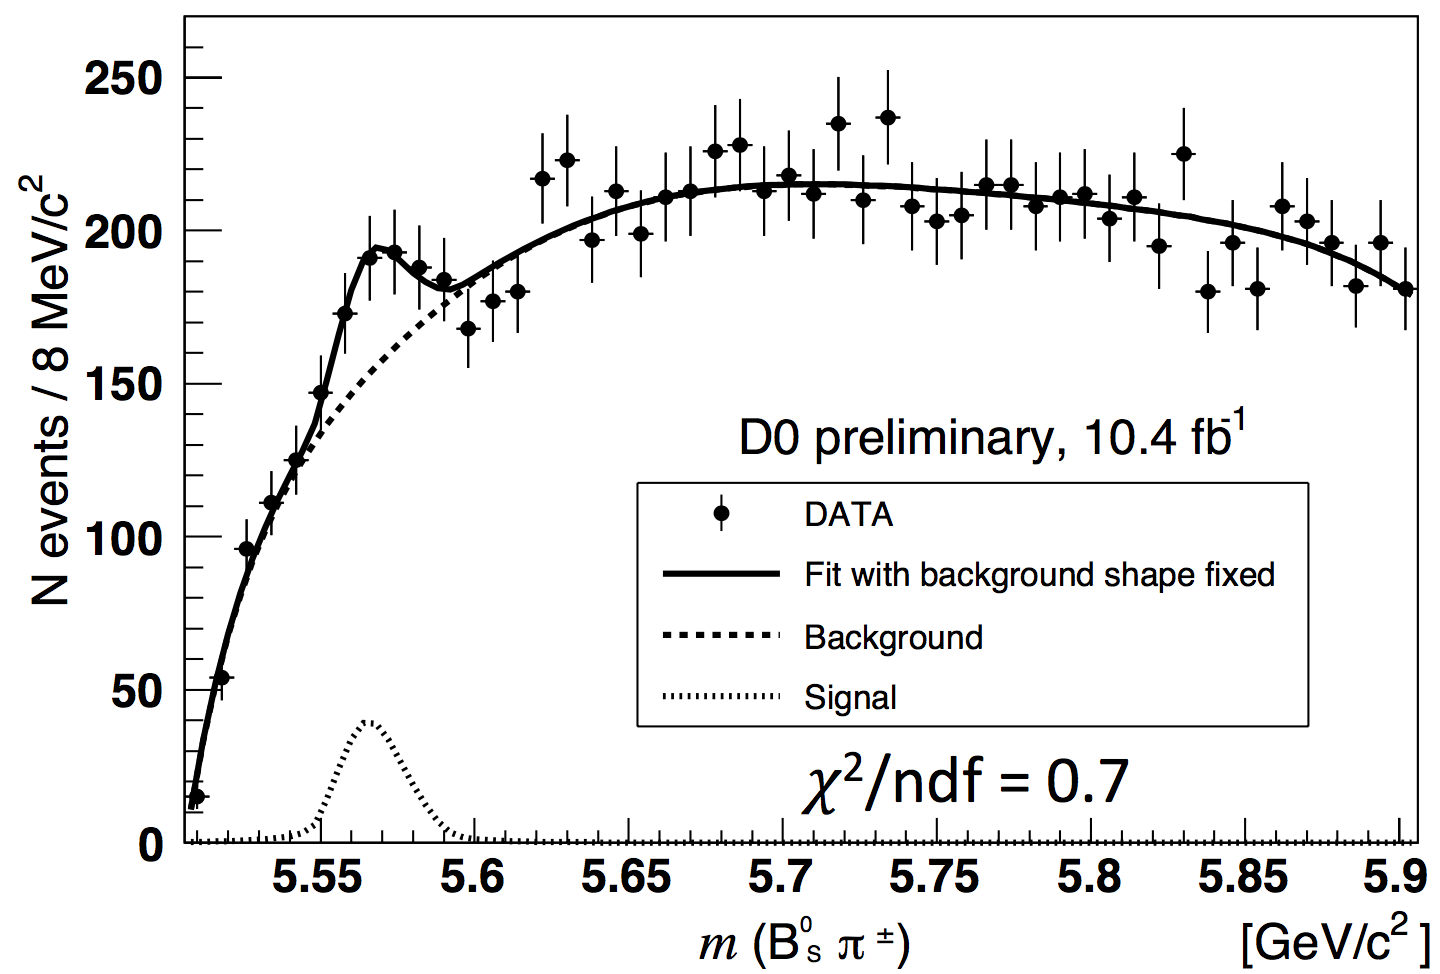
\includegraphics[width=\textwidth]{x5568_dzero.png}
    \end{column}
    \begin{column}{0.5\textwidth}
      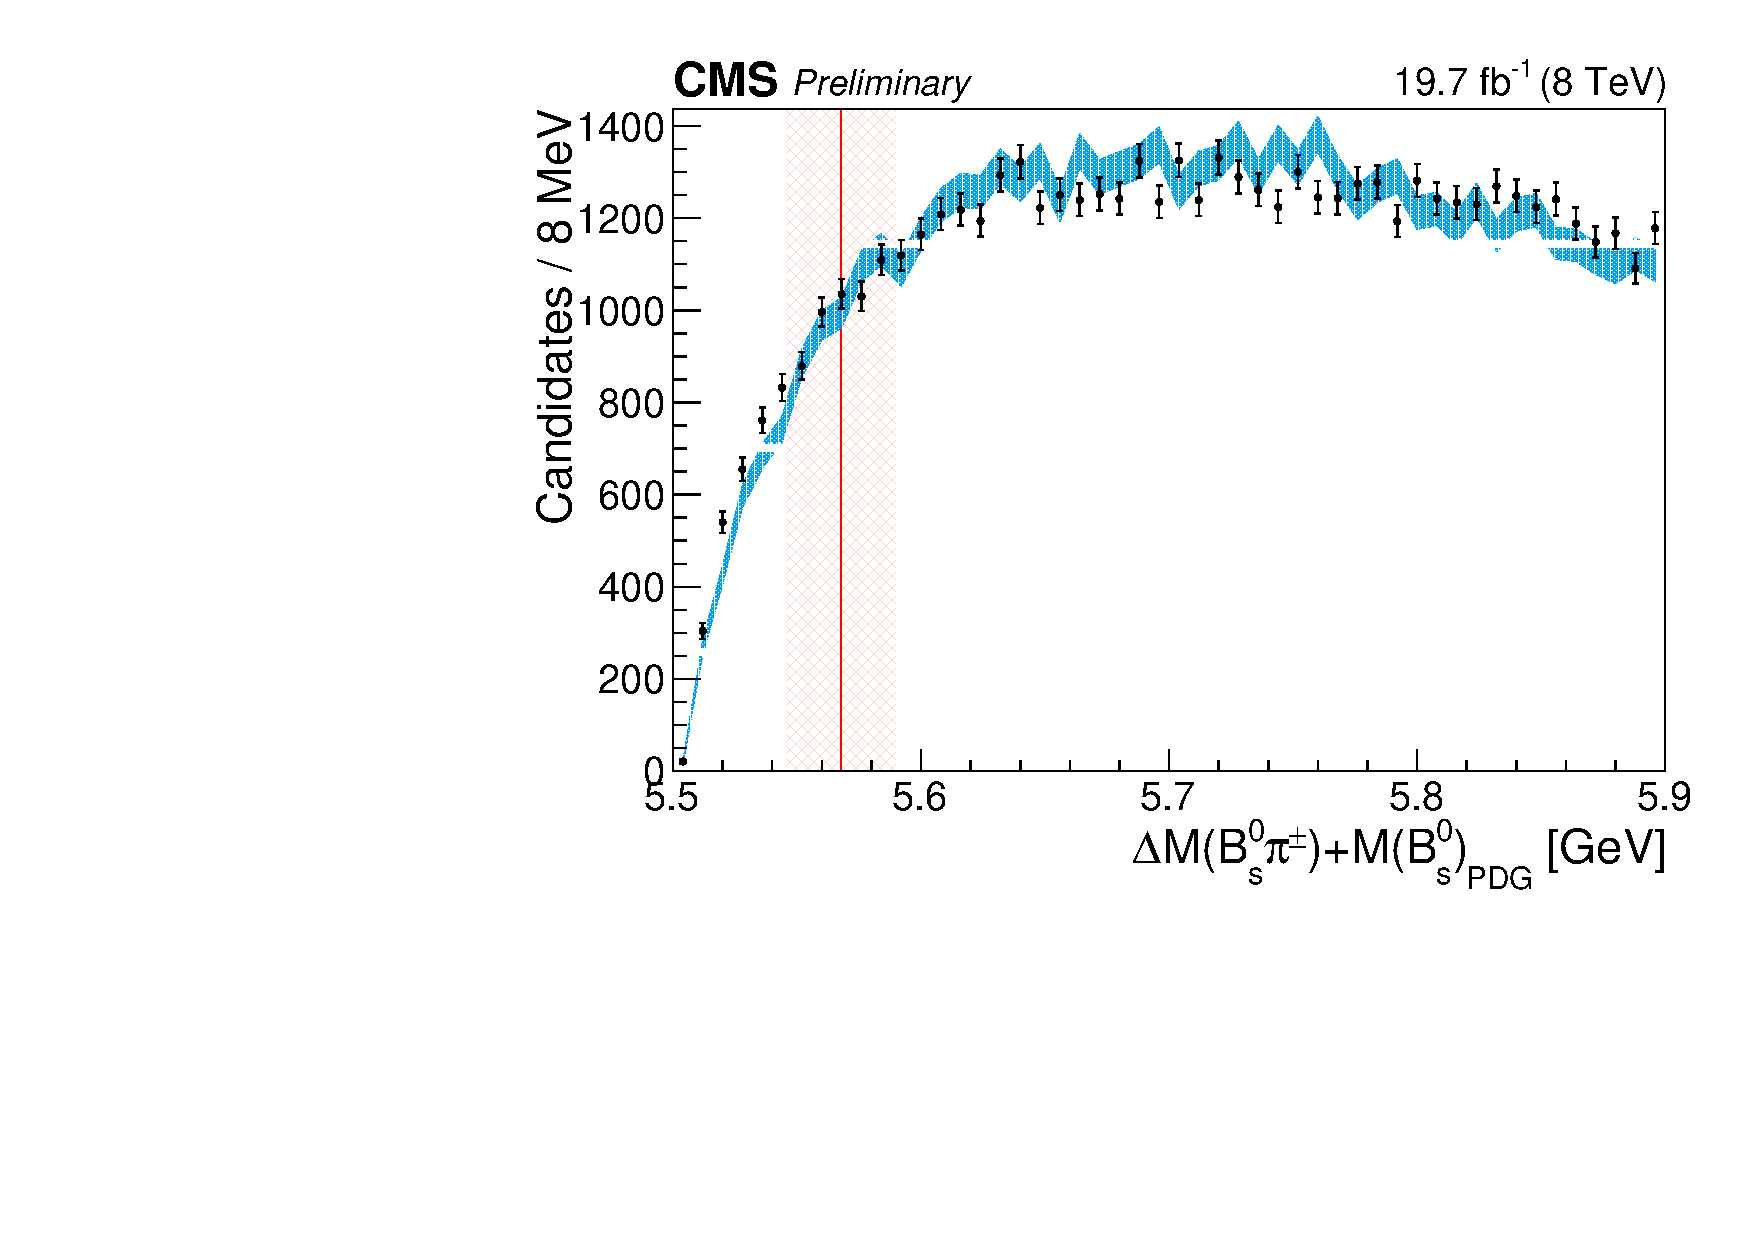
\includegraphics[width=\textwidth]{x5568_cms}
    \end{column}
  \end{columns}
  Explanation requires a significantly different production in $\proton\antiproton$ to \pp{}
\end{frame}

\section{Quarkonia}
\begin{frame}{Quarkonia%
              \righttitle{%
                \href{https://indico.cern.ch/event/568360/contributions/2486100/}{M.\ Watson},
                \href{https://indico.cern.ch/event/568360/contributions/2471879/}{J-P.\ Lansberg},
                \href{https://indico.cern.ch/event/568360/contributions/2480992/}{P.\ Ilten}
              }
             }{As a probe of double parton scattering}
  \begin{columns}
    \begin{column}{0.5\textwidth}
      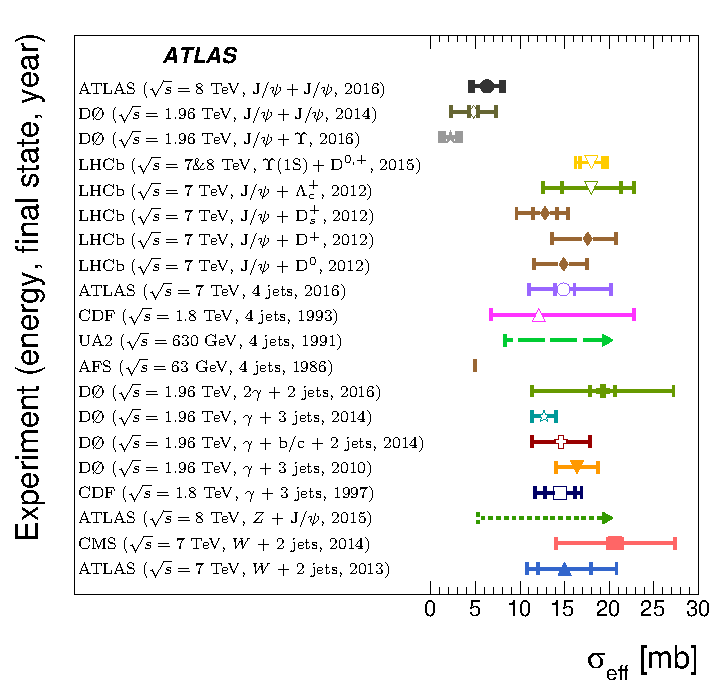
\includegraphics[width=\textwidth]{atlas_dps}
    \end{column}
    \begin{column}{0.5\textwidth}
      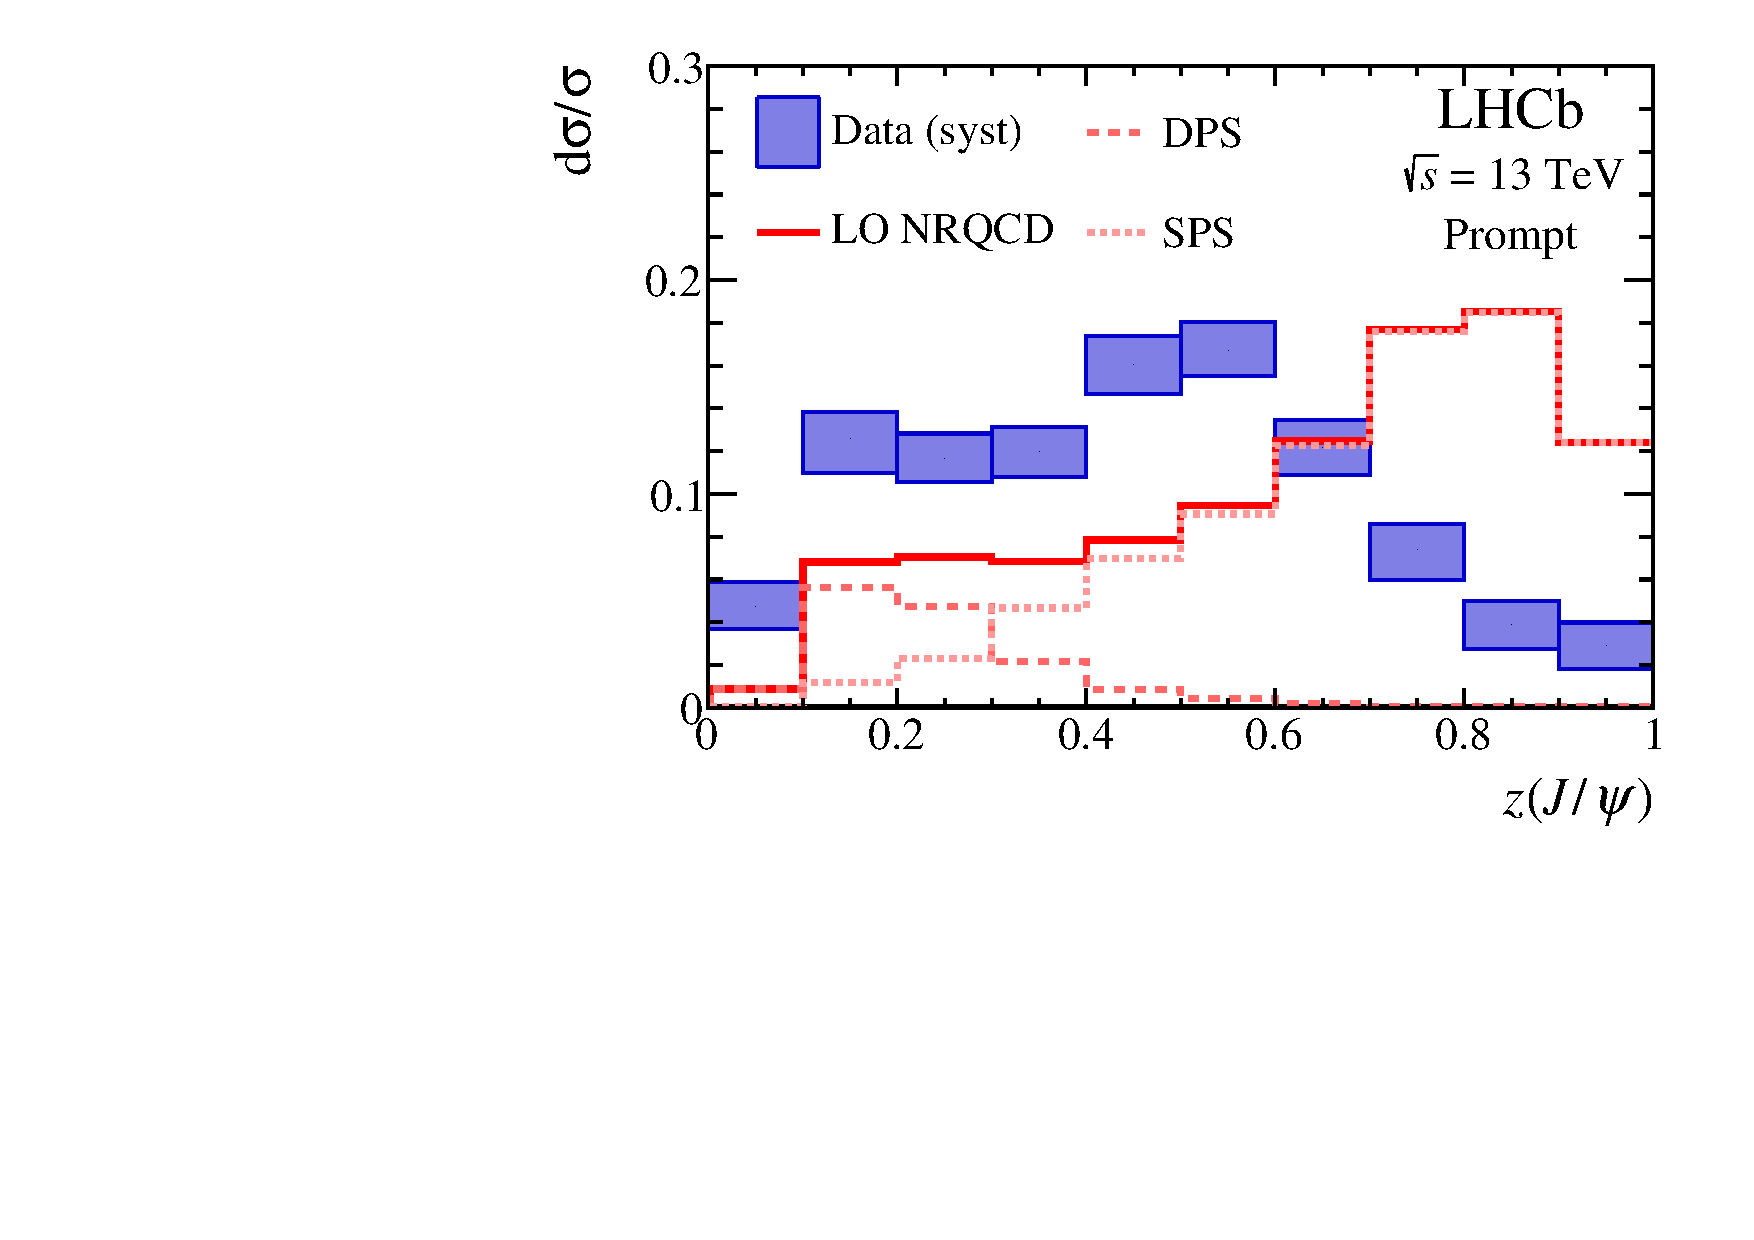
\includegraphics[width=\textwidth]{lhcb_jpsi_jets}
    \end{column}
  \end{columns}
\end{frame}

\section{Other highlights}
\begin{frame}{Other highlights}
  \begin{itemize}
    % ATLAS using b-quarks from top, CMS using triple production asymmetries of 
    % ttbar
    \item ATLAS and CMS measurements of \CP\ violation using top production
    \item CMS measurements of FCNC processes with top quarks
    \item Belle II physics programme
    \item Discussion on intrinsic charm content of proton PDF
    \item Lots of impressive theoretical progress
    \item \ldots{}plenty more
  \end{itemize}
\end{frame}

\section{Summary}
\begin{frame}{Summary}
  \begin{itemize}
    \item WG5 saw a wide variety of very interesting topics
    \item Lots of cross-pollination
      \begin{itemize}
        \item ALICE, ATLAS, CMS, and LHCb all overlap at least somewhat in most areas
        \item Other experiments providing vital input in other areas of phase space
        \item Theorists taking inputs from many more sources
        \item Experimentalists trying to provide measurements with the highest utility
      \end{itemize}
    \item Interplay of LHC heavy quark cross-section measurements with DIS is leading to greatly improved PDF precision, for better models for future colliders
  \end{itemize}
\end{frame}

\begin{frame}{Thanks}
  \begin{center}
    {\Large
    Thanks to all the speakers and participants of WG5\ldots\par
    \bigskip
    \ldots{}and to the organisers for a great conference!
    }
  \end{center}
\end{frame}

\appendix

\section{Backup}
\begin{frame}[c]
  \begin{center}
    \Huge{\structure{Backup}}
  \end{center}
\end{frame}

\end{document}
